\documentclass[UTF8]{ctexart}
\CTEXsetup[format={\Large\bfseries}]{section}
\setCJKmainfont{KaiTi}
\setmainfont{Times New Roman}
\usepackage{geometry}
\geometry{a4paper, left=3.4cm, right=3.4cm, top=2.4cm, bottom=2.4cm}
%\geometry{a4paper, scale=0.75}
%\usepackage{setspace}
%\onehalfspacing
\addtolength{\parskip}{-0.1em}
\usepackage{amsmath}
\usepackage{ulem}
\usepackage{graphicx}
\usepackage{float}
\usepackage{subfigure}
\usepackage{fancyhdr}
\pagestyle{plain}
\usepackage{caption}
\renewcommand{\figurename}{Figure}
\usepackage[colorlinks,linkcolor=blue,anchorcolor=blue, citecolor=blue, bookmarks, bookmarksopen, pdfstartview=FitH]{hyperref} 
\usepackage{listings}
\usepackage{xcolor}
\usepackage{fontspec}
\usepackage{algorithm}
\usepackage{algorithmicx}
\usepackage{algpseudocode}
\definecolor{mygreen}{rgb}{0,0.6,0}  
\definecolor{mygray}{rgb}{0.5,0.5,0.5}  
\definecolor{mymauve}{rgb}{0.58,0,0.82}  
\usepackage{diagbox}
\usepackage{multirow}
\usepackage{booktabs}

\lstset{ %  
	basicstyle={\fontspec{Consolas} \footnotesize},
	backgroundcolor=\color{white},   % choose the background color; you must add \usepackage{color} or \usepackage{xcolor}  
%	basicstyle=\footnotesize,        % the size of the fonts that are used for the code  
	breakatwhitespace=false,         % sets if automatic breaks should only happen at whitespace  
	breaklines=true,                 % sets automatic line breaking  
	captionpos=bl,                    % sets the caption-position to bottom  
	commentstyle=\color{mygreen},    % comment style  
	deletekeywords={...},            % if you want to delete keywords from the given language  
	escapeinside={\%*}{*)},          % if you want to add LaTeX within your code  
	extendedchars=true,              % lets you use non-ASCII characters; for 8-bits encodings only, does not work with UTF-8  
	frame=single,                    % adds a frame around the code  
%	keepspaces=true,                 % keeps spaces in text, useful for keeping indentation of code (possibly needs columns=flexible)  
	keywordstyle=\color{blue},       % keyword style  
	%language=Python,                 % the language of the code  
	morekeywords={*,...},            % if you want to add more keywords to the set  
	numbers=left,                    % where to put the line-numbers; possible values are (none, left, right)  
	numbersep=5pt,                   % how far the line-numbers are from the code  
	numberstyle=\tiny\color{mygray}, % the style that is used for the line-numbers  
	rulecolor=\color{black},         % if not set, the frame-color may be changed on line-breaks within not-black text (e.g. comments (green here))  
	showspaces=false,                % show spaces everywhere adding particular underscores; it overrides 'showstringspaces'  
	showstringspaces=false,          % underline spaces within strings only  
	showtabs=false,                  % show tabs within strings adding particular underscores  
	stepnumber=1,                    % the step between two line-numbers. If it's 1, each line will be numbered  
	stringstyle=\color{orange},     % string literal style  
	tabsize=2,                       % sets default tabsize to 2 spaces  
	%title=myPython.py                   % show the filename of files included with \lstinputlisting; also try caption instead of title  
}  

\makeatletter
\newenvironment{breakablealgorithm}
{% \begin{breakablealgorithm}
	\begin{center}
		\refstepcounter{algorithm}% New algorithm
		\hrule height.8pt depth0pt \kern2pt% \@fs@pre for \@fs@ruled
		\renewcommand{\caption}[2][\relax]{% Make a new \caption
			{\raggedright\textbf{\ALG@name~\thealgorithm} ##2\par}%
			\ifx\relax##1\relax % #1 is \relax
			\addcontentsline{loa}{algorithm}{\protect\numberline{\thealgorithm}##2}%
			\else % #1 is not \relax
			\addcontentsline{loa}{algorithm}{\protect\numberline{\thealgorithm}##1}%
			\fi
			\kern2pt\hrule\kern2pt
		}
	}{% \end{breakablealgorithm}
		\kern2pt\hrule\relax% \@fs@post for \@fs@ruled
	\end{center}
}
\makeatother

\makeatletter
\renewcommand{\@thesubfigure}{\hskip\subfiglabelskip}
\makeatother

\title{实验设计与数据处理}
\author{石大川 \quad 深计研211班\\ <sdc21@mails.tsinghua.edu.cn>}
\date{\today}
\begin{document}
	\maketitle
%	\tableofcontents
	\tableofcontents \newpage
	
	\section{实验背景}
	本人来自深圳国际研究生院的计算机技术专业,所在课题组的研究方向为计算机视觉。本人选取了图像分类这一计算机视觉领域具体的科研问题来进行实验的设计与数据处理。作为计算机视觉领域最经典的问题之一,图像分类的目的是训练一个模型,该模型可以将图像作为输入,并输出图像相应的类别,如:汽车,飞机,猫,狗等等。本次实验选择了ImageNet\hyperref[ref1]{[1]}作为数据集,它是计算机视觉领域最为广泛使用的数据集之一。作为大规模的图像分类数据集,ImageNet包含1281167张图像作为训练集,50000张图像作为验证集,100000张图像作为测试集。此外,本次实验选择了ResNet\hyperref[ref2]{[2]}这一计算机视觉领域引用次数最高的神经网络作为模型。具体来说,本文以ImagNet为数据集,将分辨率为$224\times 224$,也即维度数为$50176$的图像数据作为输入,训练ResNet18这一网络(ResNet18是ResNet网络的一种),该网络约有1169万的参数量。
	
	\section{实验设计}
	
	\subsection{作业要求}
	
	\begin{itemize}
		\item 对于欲研究的课题,应该采用下面实验设计方法之一采集数据,并用配套的方法分析处理数据。
		\begin{itemize}
			\item 正交实验设计
			\item 随机化(区组)实验设计
			\item 析因(因子)实验设计
			\item 响应曲面实验设计
			\item 均匀设计
			\item 其他实验设计方法
		\end{itemize} 
		\item 如果所研究实验对象确实不适合上述实验设计方法,则应采用全面实验设计方法(进行全部可能的因素的组合)并确保每种实验要重复3次及3次以上,不要使用一次改变一个因素的单因素对比法。

	\end{itemize} 
	
	\subsection{实验介绍}
	为了尽可能训练出一个准确率高的图像分类模型,我们通常需要反复调整模型中的各项超参数(hyperparameter),其中训练轮数(epoch),批处理大小(batch size)和学习率(learning rate)是三项关键的参数。在接下来的实验设计中,我们通过正交实验设计的方法,来确定关于这三个超参数的最优水平组合。
	
	\subsection{正交实验设计}
	相比于全面实验,正交实验具有减少实验次数,并且可以给出误差分析的优势,因此我们选择正交实验设计来进行相关实验。对于训练轮数,批处理大小和学习率我们根据经验各设置了3个常见的水平,如\hyperref[Chart.1]{表1}所示。为了考察实验误差,我们还需要额外的1列空列。由四因素三水平可知,最合适的正交表为$L_9(3^4)$,如\hyperref[Chart.2]{表2}所示。对照\hyperref[Chart.2]{表2},可以写出本次实验的正交实验设计表\hyperref[Chart.2]{表3}。
	
		
	\begin{table}[htbp]  
		\centering
		\caption{因素水平表} 
		\begin{center}  
			\begin{tabular}{|c|c|c|c|}  
				\hline  
				\diagbox{水平}{因素} & A:训练轮数 & B:批处理大小 & C:学习率 \\ \hline  
				1 &  16 & 8192 & 0.01  \\ \hline  
				2 & 12 & 4096 & 0.005 \\  \hline  
				3 & 8 & 2048 & 0.001\\  \hline  
			\end{tabular}  
		\end{center}  
		\label{Chart.1}
	\end{table}
	

	% Table generated by Excel2LaTeX from sheet 'Sheet1'
	\begin{table}[htbp]
		\centering
		\caption{$L_9(3^4)$表}
		\begin{tabular}{|c|c|c|c|c|}
%			\toprule
			\hline
			\multirow{2}[4]{*}{实验号} & \multicolumn{4}{c|}{列号} \\
			\cline{2-5}      & 1 & 2 & 3 & 4 \\ \hline
			1 & 1 & 1 & 1 & 1 \\ \hline
			2 & 1 & 2 & 2 & 2 \\ \hline
			3 & 1 & 3 & 3 & 3 \\
			\hline
			4 & 2 & 1 & 2 & 3 \\
			\hline
			5 & 2 & 2 & 3 & 1 \\
			\hline
			6 & 2 & 3 & 1 & 2 \\
			\hline
			7 & 3 & 1 & 3 & 2 \\
			\hline
			8 & 3 & 2 & 1 & 3 \\
			\hline
			9 & 3 & 3 & 2 & 1 \\
%			\bottomrule
			\hline
		\end{tabular}%
		\label{Chart.2}%
	\end{table}%


	\begin{table}[htbp]
		\centering
		\caption{正交实验设计表}
		\begin{tabular}{|c|c|c|c|c|c|}
%			\toprule
			\hline
			因素 & A 训练轮数 & B 批量大小 & C 学习率 &   & \multirow{2}[4]{*}{准确率(\%)} \\
			\cline{1-5} \diagbox{实验号}{列号} & 1 & 2 & 3 & 4 &  \\\hline
%			\midrule
			1 & 1(16) & 1(8192) & 1(0.01) & 1 & 59.80 \\\hline
%			\midrule
			2 & 1 & 2(4096) & 2(0.005) & 2 & 61.22 \\\hline
%			\midrule
			3 & 1 & 3(2048) & 3(0.001) & 3 & 56.86 \\\hline
%			\midrule
			4 & 2(12) & 1 & 2 & 3 & 53.76 \\\hline
%			\midrule
			5 & 2 & 2 & 3 & 1 & 44.28 \\\hline
%			\midrule
			6 & 2 & 3 & 1 & 2 & 56.34 \\\hline
%			\midrule
			7 & 3(8) & 1 & 3 & 2 & 40.61 \\\hline
%			\midrule
			8 & 3 & 2 & 1 & 3 & 53.07 \\\hline
%			\midrule
			9 & 3 & 3 & 2 & 1 & 55.23 \\\hline
%			\bottomrule
		\end{tabular}%
		\label{Chart.3}%
	\end{table}%

	\subsubsection{极差分析}
	我们需要计算$T$和$R$以确定最优水平以及主次排序。首先计算$T_{ij}$,其代表第$j$列中水平为$i$的实验结果之和。例如
	\begin{equation*}
	T_{11} = 59.80+61.22+56.86 = 177.88
	\end{equation*}
	同理可以计算得到其他的$T_{ij}$,如\hyperref[Chart.4]{表4}所示。此后通过
	\begin{equation*}
	T_{ij} = max(T_{1j}, T_{2j}, T_{3j})
	\end{equation*}
	可以得到最优水平,如A因素训练轮数的最优水平为
	\begin{equation*}
	T_{11} = max(T_{11}, T_{21}, T_{31})
	\end{equation*}
	也即$A1(16)$。此外通过
	\begin{equation*}
	R_j= max(T_{1j}, T_{2j}, T_{3j}) - min(T_{1j}, T_{2j}, T_{3j})
	\end{equation*}
	可以计算得到极差,如A因素训练轮数的极差为
	\begin{equation*}
	R_1= max(T_{11}, T_{21}, T_{31}) - min(T_{11}, T_{21}, T_{31}) = 177.88 - 148.91 = 28.97
	\end{equation*}
	将$R_j$从大到小排序,可以得到主次排序为$ACB$,且最优水平组合为$A1C2B3$。而$A1C2B3$并不是正交实验做的9个实验之一,可见虽然正交实验设计只做了局部实验,但是可以得到全局结果。
	
	使用最优水平组合$A1C2B3$再次进行实验,可以得到$63.31$的准确率,其结果高于此前9次实验中最佳组合$A1C2B2$的$61.22$。因此,最优水平组合$A1C2B3$得到了检验。
	
	此外,对比三个因素的$R_j$和空列的$R_4$可知,三个因素的$R_j$都大于空列的$R_4$,可以认为这3个因素对实验结果都存在着一定的影响。
		\begin{table}[htbp]
		\centering
		\caption{极差分析表}
		\begin{tabular}{|c|c|c|c|c|c|}
			%			\toprule
			\hline
			因素 & A 训练轮数 & B 批量大小 & C 学习率 &   & \multirow{2}[4]{*}{准确率(\%)} \\
			\cline{1-5} \diagbox{实验号}{列号} & 1 & 2 & 3 & 4 &  \\\hline
			%			\midrule
			1 & 1(16) & 1(8192) & 1(0.01) & 1 & 59.80 \\\hline
			%			\midrule
			2 & 1 & 2(4096) & 2(0.005) & 2 & 61.22 \\\hline
			%			\midrule
			3 & 1 & 3(2048) & 3(0.001) & 3 & 56.86 \\\hline
			%			\midrule
			4 & 2(12) & 1 & 2 & 3 & 53.76 \\\hline
			%			\midrule
			5 & 2 & 2 & 3 & 1 & 44.28 \\\hline
			%			\midrule
			6 & 2 & 3 & 1 & 2 & 56.34 \\\hline
			%			\midrule
			7 & 3(8) & 1 & 3 & 2 & 40.61 \\\hline
			%			\midrule
			8 & 3 & 2 & 1 & 3 & 53.07 \\\hline
			%			\midrule
			9 & 3 & 3 & 2 & 1 & 55.23 \\\hline
			%			\bottomrule
			$T_{1j}$ & 177.88 & 154.17 & 169.21 & 159.31 & \\\hline
			$T_{2j}$ & 154.38 & 158.57 & 170.21 & 158.17 & \\\hline
			$T_{3j}$ & 148.91 & 168.43 & 141.75 & 163.69 & \\\hline
			最优水平 & A1(16) & B3(2048) & C2(0.005)& & \\\hline
			$R_{j}$ & 28.97 & 14.26 & 28.46 & 5.52 & \\\hline
			主次排序 & \multicolumn{4}{c|}{ACB} & \\\hline
			
		\end{tabular}%
		\label{Chart.4}%
	\end{table}%
	
	\subsubsection{方差分析}
	极差分析具有简单直观且计算量小的优点,但是也存在着无法区分实验因素、水平引起的变化和实验误差引起
	的变化,以及不能精确估计各因素对实验结果影响的重要程度等缺点,因此我们进一步使用方差分析处理实验结果。
	
	首先根据\hyperref[Chart.4]{表4},可以计算出第$j$列水平为$i$的结果平均值:
	\begin{equation*}
	t_i = \frac{T_i}{m}
	\end{equation*}
	
	计算结果如\hyperref[Chart.5]{表5}所示。
	
	\begin{table}[htbp]
		\centering
		\caption{$t_i$计算表}
		\begin{tabular}{|c|c|c|c|c|c|}
			%			\toprule
			\hline
			因素 & A 训练轮数 & B 批量大小 & C 学习率 &   & \multirow{2}[4]{*}{准确率(\%)} \\
			\cline{1-5} \diagbox{实验号}{列号} & 1 & 2 & 3 & 4 &  \\\hline
			%			\midrule
			1 & 1(16) & 1(8192) & 1(0.01) & 1 & 59.80 \\\hline
			%			\midrule
			2 & 1 & 2(4096) & 2(0.005) & 2 & 61.22 \\\hline
			%			\midrule
			3 & 1 & 3(2048) & 3(0.001) & 3 & 56.86 \\\hline
			%			\midrule
			4 & 2(12) & 1 & 2 & 3 & 53.76 \\\hline
			%			\midrule
			5 & 2 & 2 & 3 & 1 & 44.28 \\\hline
			%			\midrule
			6 & 2 & 3 & 1 & 2 & 56.34 \\\hline
			%			\midrule
			7 & 3(8) & 1 & 3 & 2 & 40.61 \\\hline
			%			\midrule
			8 & 3 & 2 & 1 & 3 & 53.07 \\\hline
			%			\midrule
			9 & 3 & 3 & 2 & 1 & 55.23 \\\hline
			%			\bottomrule
			$T_{1j}$ & 177.88 & 154.17 & 169.21 & 159.31 & 平均值53.46\\\hline
			$T_{2j}$ & 154.38 & 158.57 & 170.21 & 158.17 & \\\hline
			$T_{3j}$ & 148.91 & 168.43 & 141.75 & 163.69 & \\\hline
			$t_{1j}$ & 59.29 & 51.39 & 56.40 & 53.10 & \\\hline
			$t_{2j}$ & 51.46 & 52.86 & 56.74 & 52.72 & \\\hline
			$t_{3j}$ & 49.64 & 56.14 & 47.25 & 54.56 & \\\hline
			
		\end{tabular}%
		\label{Chart.5}%
	\end{table}%
	
	根据公式
	\begin{equation*}
	SS_i = \frac{n}{m}\sum _{i=1}^{m}(t_i - \bar{x}^2)
	\end{equation*}
	\begin{equation*}
	f_i = m - 1
	\end{equation*}
	
	可以得到各个因素的平方和与自由度,如对于因素A迭代轮数有
	\begin{equation*}
	SS_1 = \frac{9}{3}[(59.29-53.46)^2 + (51.46-53.46)^2 + (49.64-53.46)^2] = 157.74
	\end{equation*}
	\begin{equation*}
	f_1 = 3 - 1 = 2
	\end{equation*}
	
	进而根据公式
	
	\begin{equation*}
	MS_i = \frac{SS_i}{f_i}
	\end{equation*}
	
	可以得到各个因素的均方差,如对于因素A迭代轮数有
	
	\begin{equation*}
	MS_1 = \frac{SS_1}{f_1} = \frac{157.74}{2} = 78.87
	\end{equation*}
	
	对其他因素进行同样的计算,可以得到\hyperref[Chart.6]{表6}所示的方差分析表。需要注意的是,还需要比较所有因素的$MS_i$与$MSE$,如果$MS_i < 2MSE$,则需要将$SS_i$, $f_i$和$MS_i$加入到误差项中,从而可以得到误差更正后的方差分析表,如\hyperref[Chart.7]{表7}所示。
	
	\begin{table}[htbp]
		\centering
		\caption{方差分析表(误差更正前)}
		\begin{tabular}{|c|c|c|c|}
			\hline
			方差来源 & 平方和 & 自由度 & 均方差 \\\hline
			1训练轮数 & 157.74 & 2 & 78.87 \\\hline
			2批量大小 & 35.48 & 2 & 17.74 \\\hline
			3学习率 & 173.90 & 2 & 86.95 \\\hline
			空列 & 5.66 & 2 & 2.83 \\\hline
			误差 & 5.66 & 2 & 2.83 \\\hline
		\end{tabular}%
		\label{Chart.6}%
	\end{table}%
	
	\begin{table}[htbp]
		\centering
		\caption{方差分析表(误差更正后)}
		\begin{tabular}{|c|c|c|c|}
			\hline
			方差来源 & 平方和 & 自由度 & 均方差 \\\hline
			1训练轮数 & 157.74 & 2 & 78.87 \\\hline
			2批量大小 & 35.48 & 2 & 17.74 \\\hline
			3学习率 & 173.90 & 2 & 86.95 \\\hline
			空列 & 5.66 & 2 & 2.83 \\\hline
			误差 & 5.66 & 2 & 2.83 \\\hline
			总和 & 372.78 & 8 & \\\hline
		\end{tabular}%
		\label{Chart.7}%
	\end{table}%
	
	此后根据公式
	\begin{equation*}
	F_i = \frac{MS_i}{MSE}
	\end{equation*}
	
	可以计算得到F值,如对于因素A训练轮数有
	\begin{equation*}
	F_1 = \frac{MS_1}{MSE} = \frac{78.87}{2.83} = 27.87
	\end{equation*}
	
	通过查阅F临界值表,可以得到最终的方差分析\hyperref[Chart.8]{表8}。可见因素训练轮数和因素学习率的F值都超过了$F_{0.05}(2, 2)$,但是没有超过$F_{0.01}(2, 2)$,因此可以认为因素训练轮数和因素学习率都是显著的。而因素批量大小的F值没有超过$F_{0.05}(2, 2)$,因此可以认为因素批量大小不显著。
	
	此外,通过方差分析给出的主次顺序为CAB,这与极差分析给出的主次顺序ACB在第一次序和第二次序上有所不同。
	
	\begin{table}[htbp]
		\centering
		\caption{方差分析表}
		\begin{tabular}{|c|c|c|c|c|c|c|}
			\hline
			方差来源 & 平方和 & 自由度 & 均方差 & F值 & $F_{\alpha}$ & 显著性 \\\hline
			1训练轮数 & 157.74 & 2 & 78.87 & 27.87 & $F_{0.05}(2, 2)=19.00$ & $*$\\\hline
			2批量大小 & 35.48 & 2 & 17.74 & 6.27 & &  \\\hline
			3学习率 & 173.90 & 2 & 86.95 & 30.72 & $F_{0.05}(2, 2)=19.00$ & $*$ \\\hline
			空列 & 5.66 & 2 & 2.83 & & & \\\hline
			误差 & 5.66 & 2 & 2.83 & & & \\\hline
			总和 & 372.78 & 8 & & & & \\\hline
		\end{tabular}%
		\label{Chart.8}%
	\end{table}%

	\subsubsection{使用DesignExpert软件验证}
	
	在DesignExpert软件中选择Taguchi OA(田口正交阵列),进行正交实验的设计和分析。选择$L_9(3^4)$正交表后将3个因素和各自的3个水平输入到因素水平表中,如\hyperref[Fig.1]{图1}所示。
	
	\begin{figure}[htbp]
		\centering
		\caption{因素水平表}
		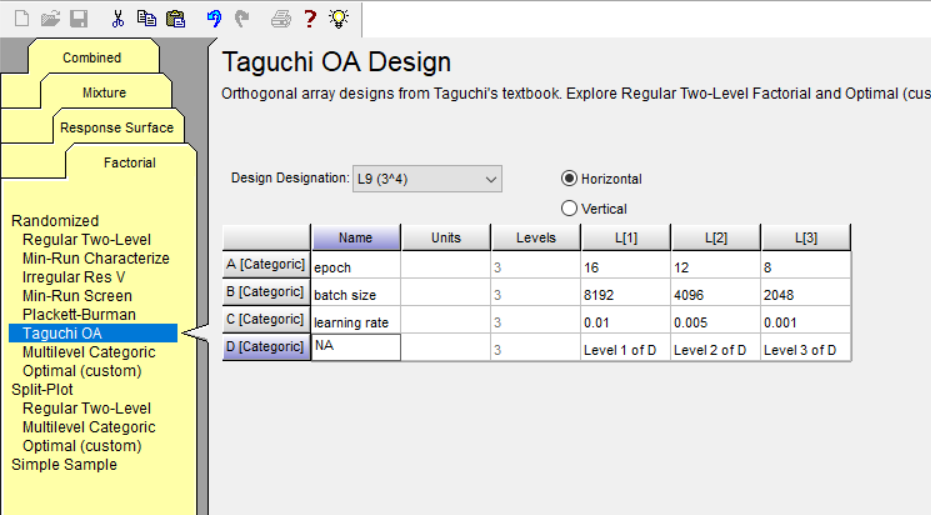
\includegraphics[width=1.0\textwidth]{pic1.png}
		\label{Fig.1}
	\end{figure}
	
	接下来,由于正交设计不适合分析交互作用和高阶,我们使用默认的只分析一阶效应的选项。在生成实验设计表后,填入\hyperref[Chart.3]{表3}中的实验数据,如\hyperref[Fig.2]{图2}所示。
	
	\begin{figure}[htbp]
		\centering
		\caption{正交实验设计表}
		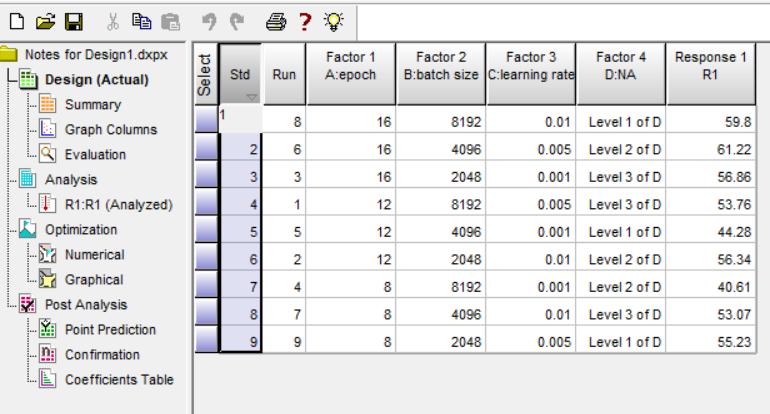
\includegraphics[width=1.0\textwidth]{pic5.png}
		\label{Fig.2}
	\end{figure}
	
	在Effect页面,可以发现在3个实验因素中,因素A训练轮数和因素C学习率效果较明显,而因素B批处理大小效果较不明显,如\hyperref[Fig.3]{图3}所示。图中离直线越远说明效果越明显。
	
	\begin{figure}[htbp]
		\centering
		\caption{Effect页面}
		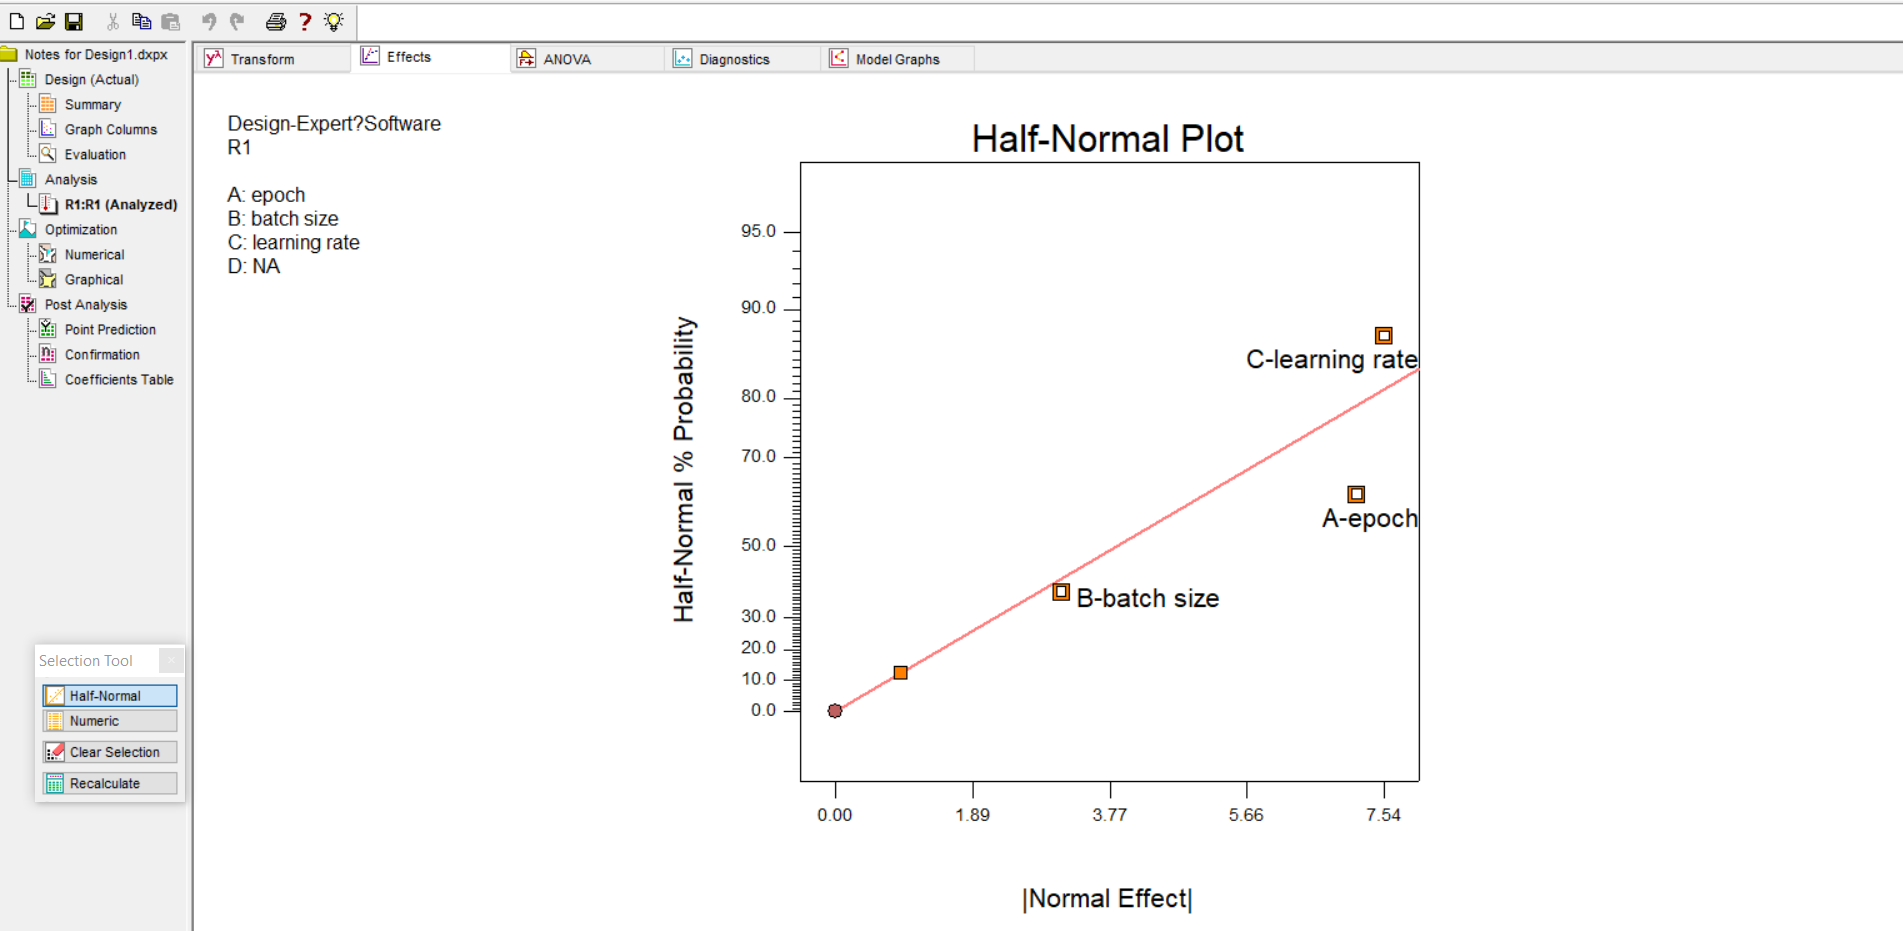
\includegraphics[width=1.0\textwidth]{pic6.png}
		\label{Fig.3}
	\end{figure}

	在Selection Tool中选择Numeric可以看到DesignExpert软件计算出的各因素的平方和,自由度和均方差,如\hyperref[Fig.4]{图4}所示。将其结果与\hyperref[Chart.7]{表7}的计算结果对比可知,在舍入误差允许的范围内,可以认为计算结果是正确的。
	
	\begin{figure}[htbp]
		\centering
		\caption{数值计算结果}
		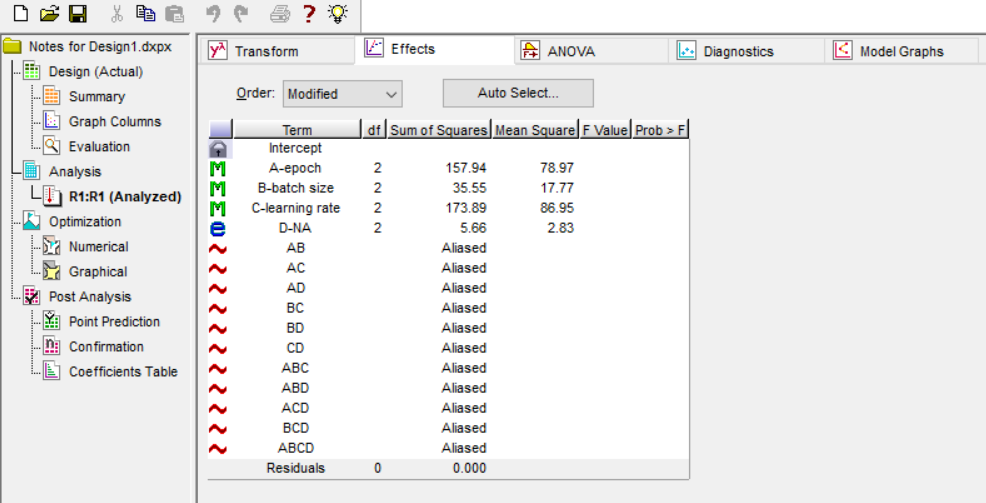
\includegraphics[width=1.0\textwidth]{pic7.png}
		\label{Fig.4}
	\end{figure}

	最后选择ANOVA页面,可以看到DesignExpert软件完成的方差分析,\hyperref[Fig.5]{图5}所示。对比\hyperref[Chart.8]{表8}的计算结果可知,在舍入误差允许的范围内,可以认为计算结果是正确的。此外DesingExpert软件也给出了训练轮数,批处理大小和学习率三个因素构成的模型总体上显著的结论。具体来说,对于因素C学习率,只有$3.15\% < 5\%$的概率因素C学习率的F值偏大是因为噪声,因此因素C学习率是显著的;对于因素A训练轮数,只有$3.46\% < 5\%$的概率因素A训练轮数的F值偏大是因为噪声,因此因素A训练轮数是显著的;对于因素B批处理大小,有$13.74\% < 5\%$的概率因素B批处理大小的F值偏大是因为噪声,因此因素B批处理大小不显著;总体而言,由训练轮数,批处理大小和学习率三个因素构成的模型只有$4.48\% < 5\%$的概率其F值偏大是因为噪声,因此三个因素构成的模型总体上是显著的。
	
	\begin{figure}[htbp]
		\centering
		\caption{方差分析结果}
		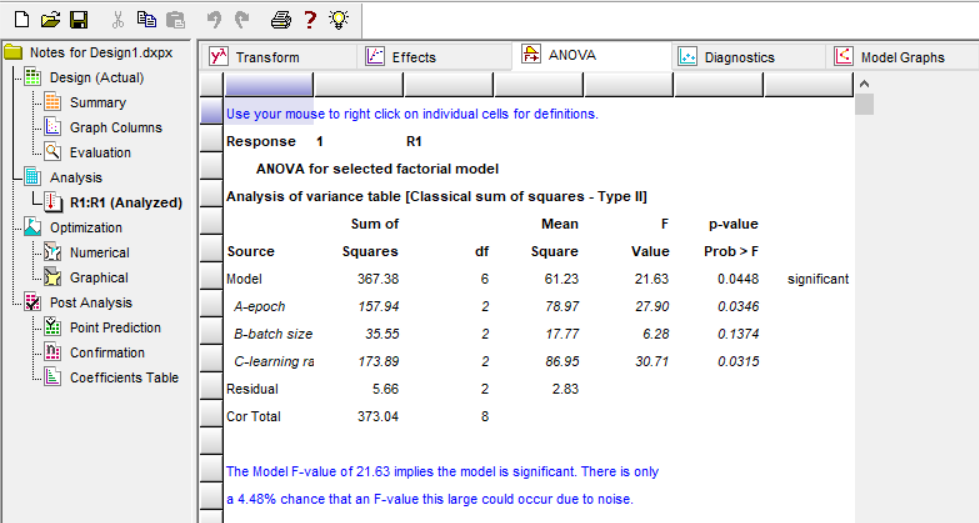
\includegraphics[width=1.0\textwidth]{pic8.png}
		\label{Fig.5}
	\end{figure}
	
	鉴于我们发现因素B批处理大小不显著,我们在Effect中手动去掉因素B批处理大小,如\hyperref[Fig.6]{图6}所示。
	
	\begin{figure}[htbp]
		\centering
		\caption{Effect页面(不选择因素B批处理大小)}
		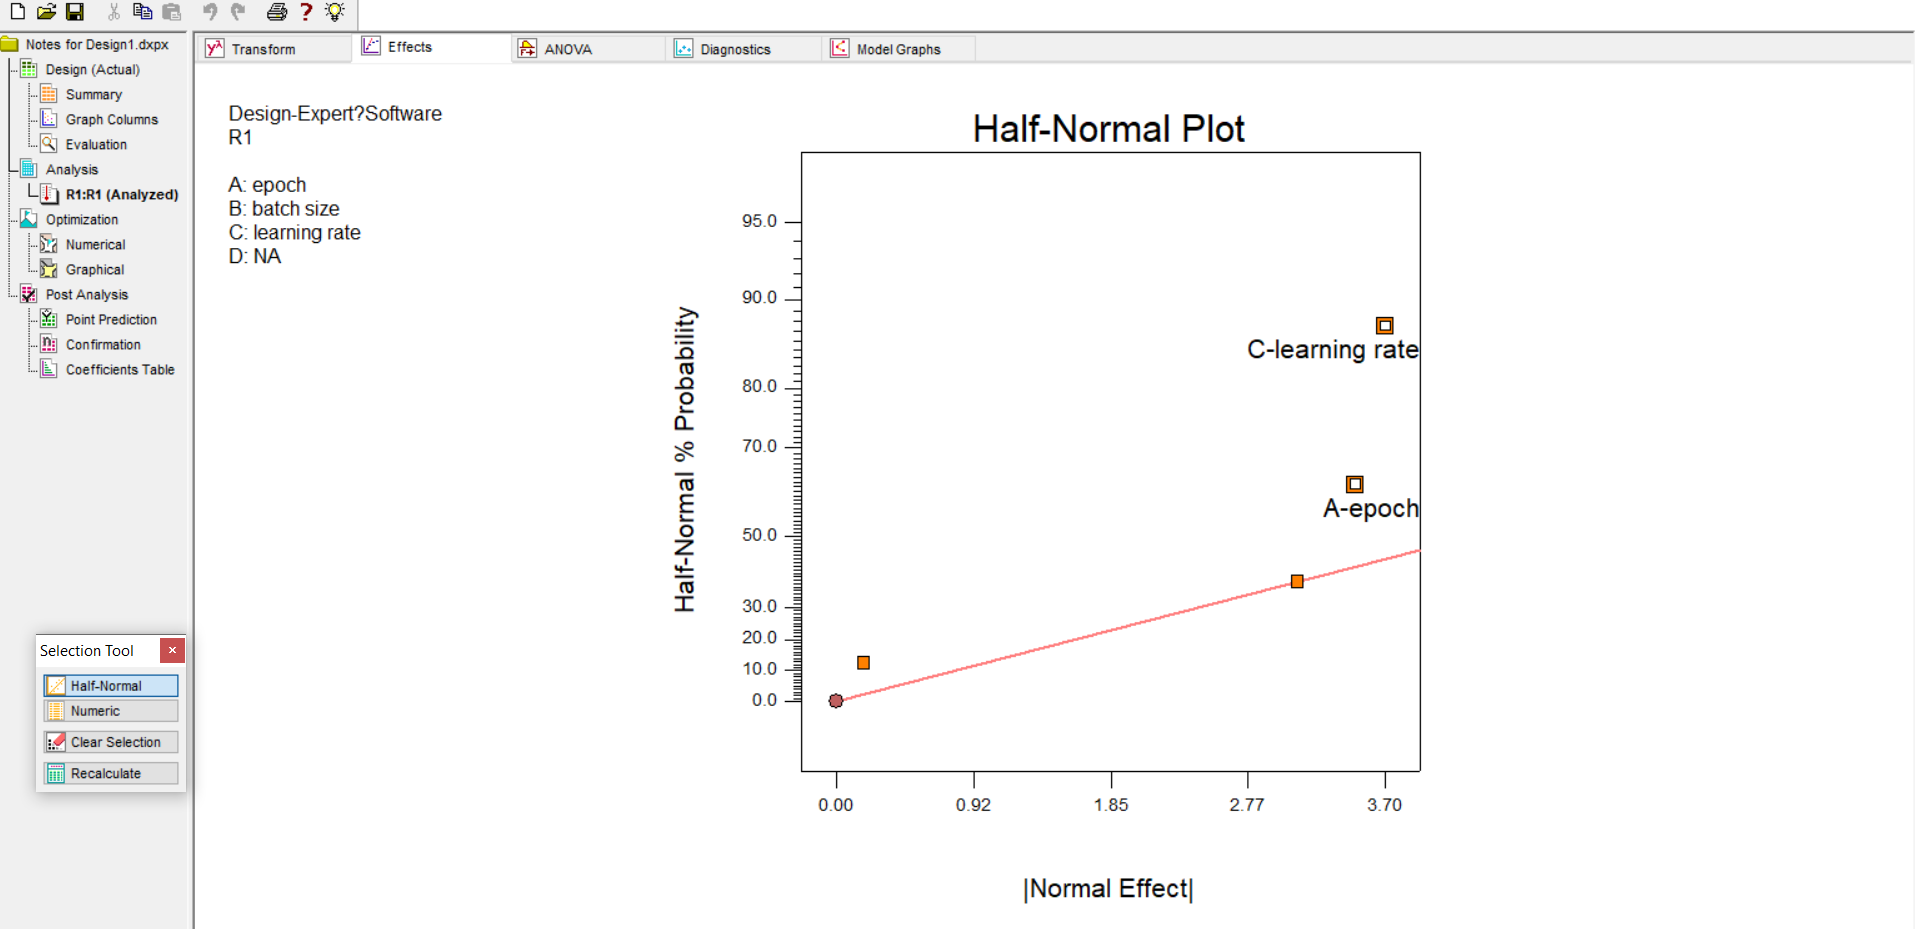
\includegraphics[width=1.0\textwidth]{pic9.png}
		\label{Fig.6}
	\end{figure}

	相应地,只包含因素C学习率和因素A训练轮数的方差分析结果如\hyperref[Fig.7]{图7}所示。
		
	\begin{figure}[htbp]
		\centering
		\caption{方差分析结果(只包含因素C学习率和因素A训练轮数)}
		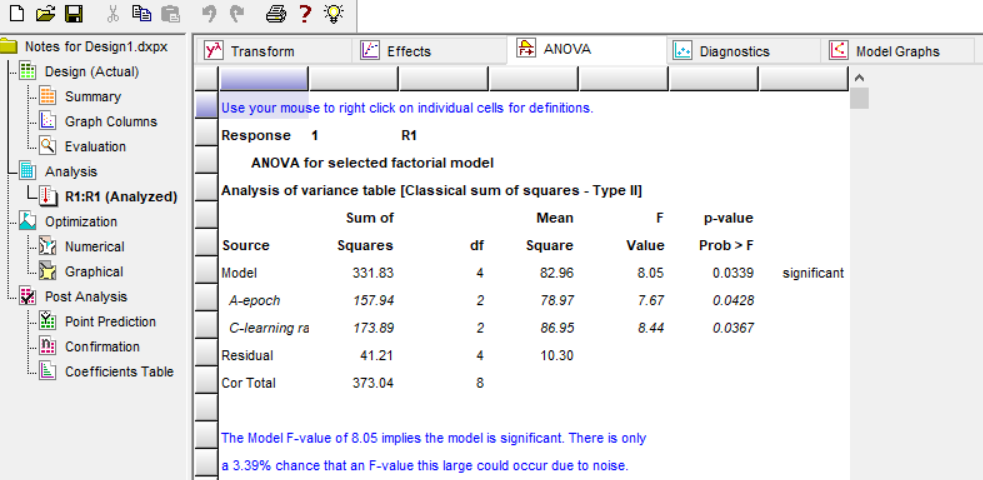
\includegraphics[width=1.0\textwidth]{pic10.png}
		\label{Fig.7}
	\end{figure}
	
	可见两因素模型总体上仅有$3.39\%$的概率其F值偏大是因为噪声,比三因素分析中总体$4.48\%$的概率更加显著。
	
	\subsubsection{正交实验设计总结}
	
	首先,对于三因素三水平的实验,如果采用全面实验法需要进行$27$次实验,而使用正交实验法则仅需要$9$次实验,节省了$27-9=18$次实验的工作量。
	
	从实验结果的极差分析可知,虽然正交实验只做了局部实验,但是可以得到全局结果。根据实验验证,由正交实验设计推理出的最优水平组合确实比9次正交实验中的最佳组合效果更好。
	
	从实验结果的方差分析可知,因素C学习率和因素A训练轮数是显著因素,在训练模型时我们应当更加关注这两个因素。而因素B批处理大小是不显著因素,在训练模型时我们不必过多关注这个因素。
	
	此外需要说明的是,本次实验得到的关于三个因素各自显著性的结论只针对在ImageNet数据集上训练的ResNet18模型成立,对于其他的数据集和模型不一定成立。尤其是对于批处理大小这个因素,在我们的实验中其效果不显著的原因可能是,为了快速训练完模型,我们选择了超大的批处理大小($2048 \sim 8192$),然而当批处理大小较小(如$<100$)时,有诸多研究表明批处理大小对于实验结果会产生显著影响。
	
	
	\section{数据的预处理和统计分析}
	
	\subsection{作业要求}
	
	\begin{itemize}
		\item 样本数量不得少于30个,各样本数据维度不得少于两维
		\item 对所获得数据进行数据预处理,给出样本的
		\begin{itemize}
			\item 均向量
			\item 协方差矩阵
			\item 相关系数矩阵
			\item 变量的直方图,箱式图
			\item 对各变量的异常数据进行判别和取舍
		\end{itemize} 
		\item  对预处理的数据完成以下统计分析之一(四选一),并简述分析的具体过程、方法以及检验(或分析方法)的意义。
		\begin{itemize}
			\item 数据的分布检验
			\item 参数估计
			\item 统计检验
			\item 方差分析(或极差分析)
		\end{itemize} 
	
	\end{itemize} 

	\subsection{实验介绍}
	在数据的预处理和统计分析中,我们从ImageNet数据集中随机选择了10000张图片做为实验数据。对于每张图片,通过图像处理可以获得\hyperref[Chart.9]{表9}中的7项特征。因此总体的实验数据为$10000 \times 7$的矩阵,部分特征数据如\hyperref[Fig.8]{图8}所示。
	
	\begin{table}[htbp]
		\centering
		\caption{实验数据的7项特征}
		\begin{tabular}{ccc}
			\toprule
			特征 & 含义 & 取值范围 \\
			\midrule
			R & Red: 图像在RGB色彩空间的R分量 & [0,255] \\
			\midrule
			G & Green: 图像在RGB色彩空间的G分量 & [0,255] \\
			\midrule
			B & Blue: 图像在RGB色彩空间的B分量 & [0,255] \\
			\midrule
			Gr & Gray: 图像的灰度分量 & [0,255] \\
			\midrule
			H & Hue: 图像在HSV色彩空间的色相分量 & [0,180] \\
			\midrule
			S & Saturation: 图像在HSV色彩空间的饱和度分量 & [0,255] \\
			\midrule
			V & Value: 图像在HSV色彩空间的明度分量 & [0,255] \\
			\bottomrule
		\end{tabular}%
		\label{Chart.9}%
	\end{table}%

	\begin{figure}[htbp]
		\centering
		\caption{部分特征数据图示}
		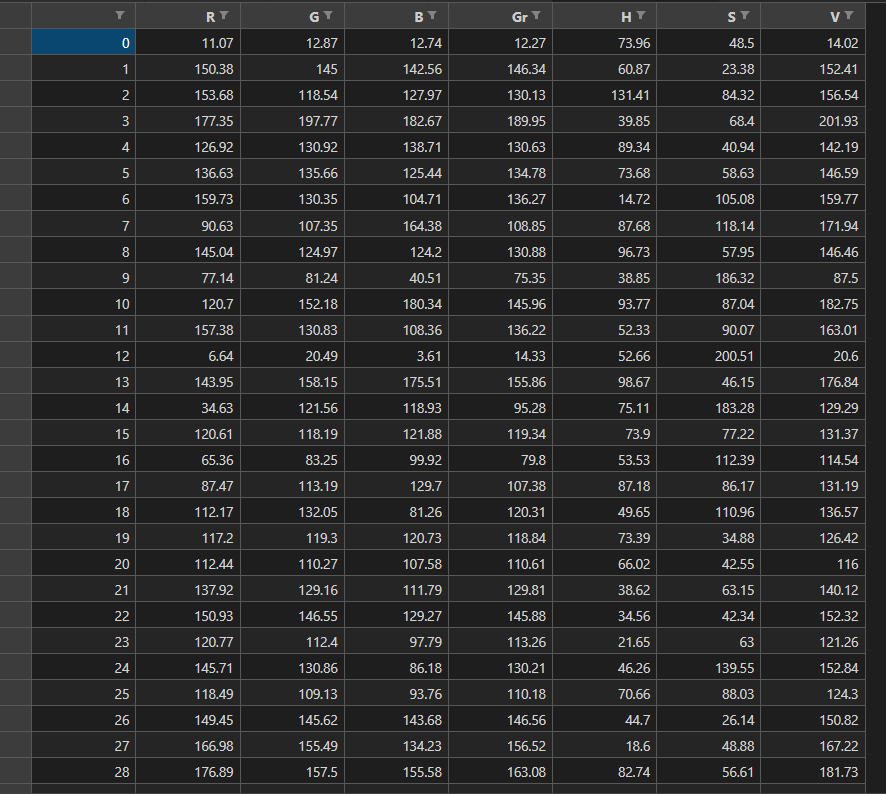
\includegraphics[width=1.0\textwidth]{data_csv.png}
		\label{Fig.8}
	\end{figure}

	\subsection{数据的预处理}
	
	\subsubsection{均向量}
	设$x_{ij}$代表实验数据中第$i$个样本的第$j$个特征的值,$n$代表实验的样本量。则第$j$个特征的平均值可以根据
	\begin{equation*}
	\bar{x}_j = \sum_{i=1}^{n}x_{ij}
	\end{equation*}
	
	得到。经计算可得实验数据的均向量为:
	\begin{equation*}
	\bar{x} = 
	\begin{bmatrix}
	120.61 &114.73& 102.39 &115.08  &53.34  &84.22 &131.77
	\end{bmatrix}
	\end{equation*}

	\subsubsection{协方差矩阵}
	
	任意两个特征之间的协方差可以根据
	\begin{equation*}
	cov(x_j, x_{j'}) = \frac{\sum_{i=1}^{n} (x_{ij} - \bar{x}_j)(x_{ij'} - \bar{x}_{j'})}{n-1}
	\end{equation*}
	
	得到,其中$j$和$j'$代表$cov(x_j, x_{j'})$是协方差矩阵中第$j$行第$j'$列的元素。经计算可得实验数据的协方差矩阵为:
	\begin{equation*}
	\Sigma = 
	\begin{bmatrix}
	1370.05 & 1085.61  & 955.77 & 1155.93 & -149.01 & -465.24 & 1176.62 \\
	1085.61 & 1253.07 & 1222.92 & 1199.58  &  38.43 & -633.86 & 1152.69 \\
	955.77 & 1222.92 & 1654.07 & 1192.19 &  369.7 & -1024.59 & 1167.12 \\
	1155.93 & 1199.58 & 1192.19 & 1185.72  &  20.08 & -628.02 & 1161.52 \\
	-149.01  &  38.43 &  369.7  &   20.08 &  697.04 & -133.64  &  75.12 \\
	-465.24 & -633.86 & -1024.59 & -628.02 & -133.64 & 2029.85 & -228.16 \\ 
	1176.62 & 1152.69 & 1167.12 & 1161.52  &  75.12 & -228.16 & 1300.92 \\
	\end{bmatrix}
	\end{equation*}
	
	\subsubsection{相关系数矩阵}
	相比于协方差矩阵,相关系数矩阵考虑了各个特征的数值在尺度上的差异,其元素取值范围为$[-1, 1]$,其值越大代表正相关性越强,其值越小代表负相关性越强。相关系数矩阵可以根据
	\begin{equation*}
	corr(x_j, x_{j'}) = \frac{cov(x_j, x_{j'})}{\sqrt{cov(x_j, x_j)} \times \sqrt{cov(x_{j'}, x_{j'})}}
	\end{equation*}
	
	得到,其中$j$和$j'$代表$corr(x_j, x_{j'})$是相关系数矩阵中第$j$行第$j'$列的元素。经计算可得实验数据的相关系数矩阵为:
	\begin{equation*}
	R = 
	\begin{bmatrix}
	1.00 &   0.83 & 0.63 & 0.91& -0.15& -0.28 & 0.88 \\
	0.83 & 1.00  &  0.85 & 0.98 & 0.04& -0.40 &  0.90 \\
	0.63 & 0.85 & 1.00  &  0.85 & 0.34& -0.56 & 0.80 \\
	0.91 & 0.98 & 0.85 & 1.00  &  0.02 &-0.40 & 0.94 \\
	-0.15 & 0.04 & 0.34 & 0.02 & 1.00 &  -0.11&  0.08 \\
	-0.28 & -0.40 & -0.56 & -0.40 & -0.11 & 1.00 &  -0.14 \\
	0.88 & 0.90  & 0.80  & 0.94 & 0.08 & -0.14 & 1.00 \\
	\end{bmatrix}
	\end{equation*}
	
	该相关系数矩阵的热力图如\hyperref[Fig.9]{图9}所示。从相关系数矩阵及其热力图可以得到以下结论:
	\begin{itemize}
		\item $R$, $G$, $B$, $Gr$和$V$这五个特征之间具有较强的正相关性。
		\item $H$和$S$这两个特征之间,以及与其他变量之间的相关性都较弱。
		\item 特征两两之间除自相关外,最强的正相关性出现在特征$G$和$Gr$之间,相关系数为$0.98$。
		\item 特征两两之间除自相关外,最强的负相关性出现在特征$B$和$S$之间,相关系数为$-0.56$。
		\item 特征两两之间最弱的相关性出现在特征$Gr$和$H$之间,相关系数的绝对值仅为$0.02$。
	\end{itemize} 
	
	\begin{figure}[htbp]
		\centering
		\caption{相关系数矩阵的热力图}
		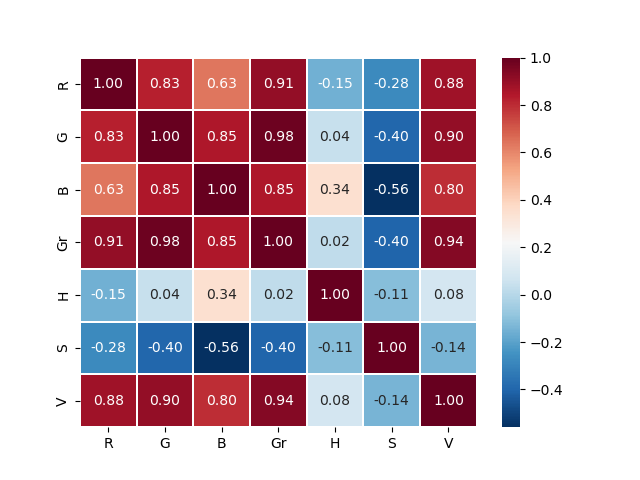
\includegraphics[width=1.0\textwidth]{heatmap.png}
		\label{Fig.9}
	\end{figure}
	
	\subsubsection{变量的直方图}
	
	对于每个特征,我们分别绘制出它的直方图。分别如\hyperref[Fig.10]{图10},\hyperref[Fig.11]{图11},\hyperref[Fig.12]{图12}和\hyperref[Fig.13]{图13}所示。从这些直方图中可以发现,特征$R$, $G$, $Gr$和$V$呈正态分布;特征$B$呈轻微右偏分布;特征$H$和$S$呈明显右偏分布。
	
	\begin{figure}[htbp]
		\centering 
		\caption{特征R和特征G的直方图}
		\subfigure[特征R的直方图]{
			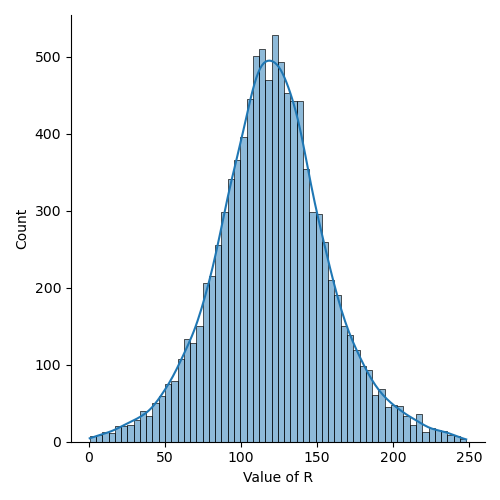
\includegraphics[width=0.49\textwidth]{hist_r.png}}
		\subfigure[特征G的直方图]{
			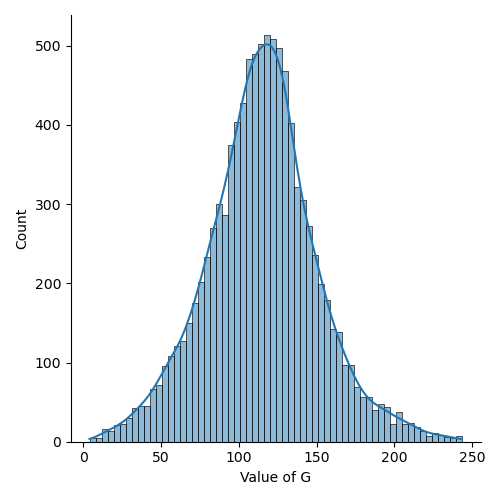
\includegraphics[width=0.49\textwidth]{hist_g.png}}
		\label{Fig.10}
	\end{figure}
	
	\begin{figure}[htbp]
		\centering 
		\caption{特征B和特征Gr的直方图}
		\subfigure[特征B的直方图]{
			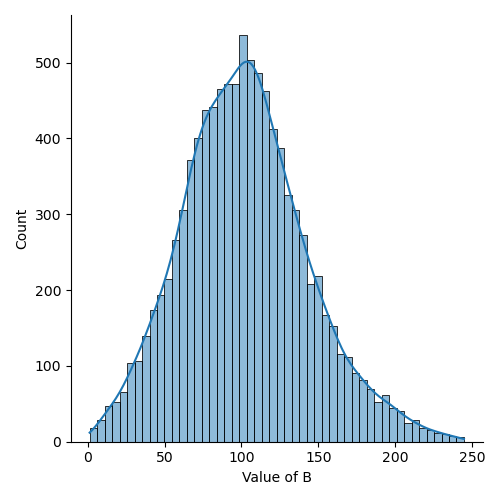
\includegraphics[width=0.49\textwidth]{hist_b.png}}
		\subfigure[特征Gr的直方图]{
			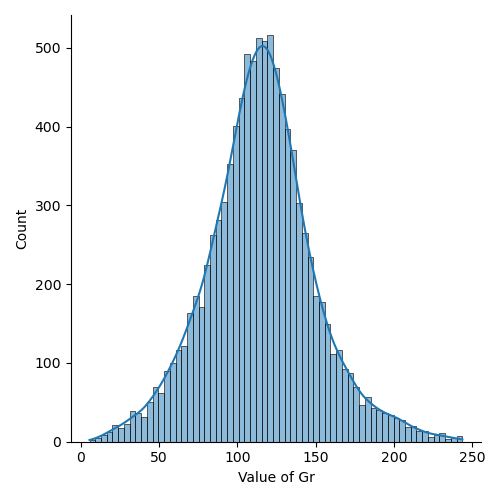
\includegraphics[width=0.49\textwidth]{hist_gr.png}}
		\label{Fig.11}
	\end{figure}

	\begin{figure}[htbp]
	\centering 
	\caption{特征H和特征S的直方图}
	\subfigure[特征H的直方图]{
		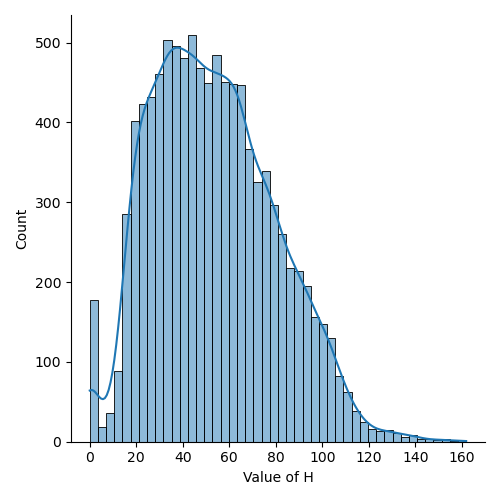
\includegraphics[width=0.49\textwidth]{hist_h.png}}
	\subfigure[特征S的直方图]{
		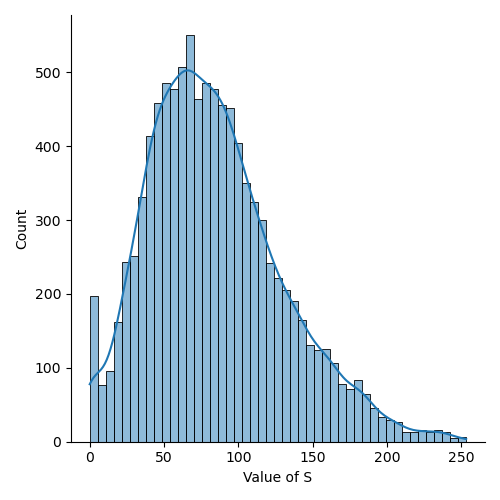
\includegraphics[width=0.49\textwidth]{hist_s.png}}
	\label{Fig.12}
	\end{figure}

	\begin{figure}[htbp]
	\centering
	\caption{特征V的直方图}
	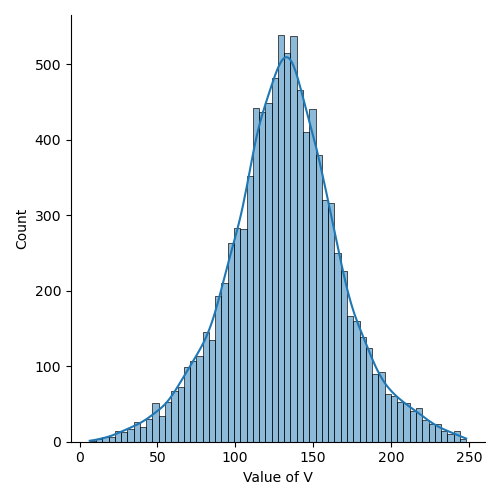
\includegraphics[width=0.5\textwidth]{hist_v.png}
	\label{Fig.13}
	\end{figure}

	\subsubsection{变量的箱式图}
	
	箱式图可以反映数据的分布情况。每个箱型中包含5条横线,从上到下依次代表上边缘,上四分位数,中位数,下四分位数和下边缘。此外处于上边缘以上和下边缘以下的数据点我们将它们当作异常值。为了方便综合比较,我们将七个特征的箱式图绘制在一张图中,如\hyperref[Fig.14]{图14}所示。
	
	从箱式图中可以看出:
	\begin{itemize}
		\item 七个特征的箱体都较窄,说明正常数据在中位数附近较为集中。
		\item $R$, $G$, $B$, $Gr$和$V$这五个特征的分布较为接近。
		\item $H$和$S$两个特征之间,以及与其他特征之间的分布相差较大。
		\item $H$和$S$两个特征的中位数分别更靠近它们箱体的下沿,呈右偏分布。
		\item 七个特征都有异常值,其中特征$B$, $H$和$S$只有大于上边缘的异常值,而没有小于下边缘的异常值。
	\end{itemize} 

	\begin{figure}[htbp]
		\centering
		\caption{七个特征的箱式图}
		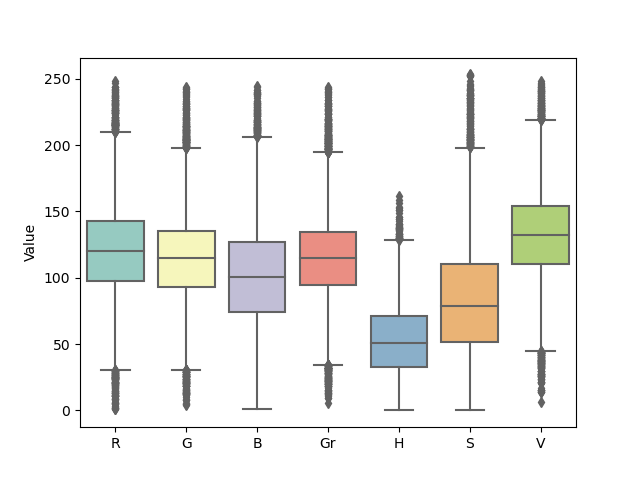
\includegraphics[width=1.0\textwidth]{box_plot.png}
		\label{Fig.14}
	\end{figure}
	
	\subsubsection{对各变量的异常数据进行判断和取舍}
	
	有多种方法可以对异常数据进行判断和取舍,如散点图法,箱型图法和置信区间法等等。
	
	\paragraph{散点图法} 我们先做出数据的散点图,将图中明显不符合其他数据模型的点判定为异常数据。以特征$H$为例,其散点图如\hyperref[Fig.15]{图15}所示。从图中可以看出,图的顶部有数个明显离群的点,我们可以认为这些点是异常数据。
	
	\begin{figure}[htbp]
		\centering
		\caption{特征$H$的散点图}
		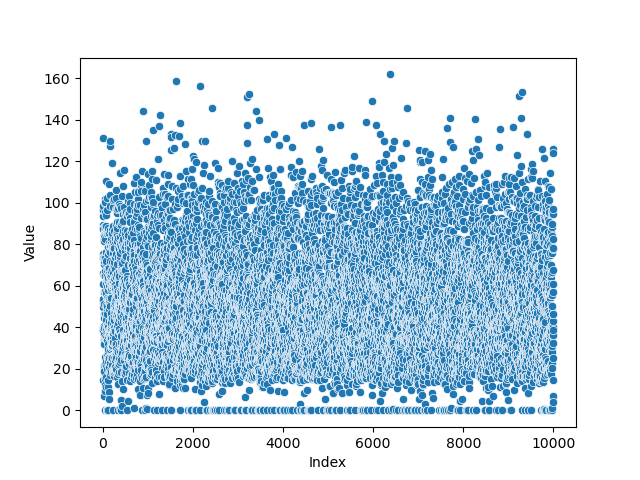
\includegraphics[width=1.0\textwidth]{scatter_h.png}
		\label{Fig.15}
	\end{figure}
	
	\paragraph{箱型图法} 我们先做出数据的箱型图,记上四分位数为$Q3$,下四分位数为$Q1$,上下四分位数的差值为$IQR$,则我们将大于$Q3+1.5IQR$或者小于$Q1-1.5IQR$的值定义为奇异点。同样以特征$H$为例,其箱型图如\hyperref[Fig.16]{图16}所示。从图中可以看出,特征$H$的数值大于$130$的点可以认为是异常数据。
	
	\begin{figure}[htbp]
		\centering
		\caption{特征$H$的箱型图}
		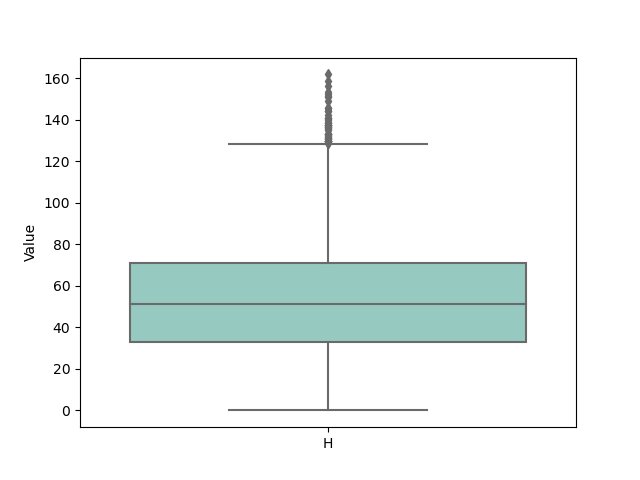
\includegraphics[width=1.0\textwidth]{box_h.png}
		\label{Fig.16}
	\end{figure}
	
	
	\paragraph{置信区间法} 置信区间法以统计量的置信上限和置信下限作为上下界构成置信区间,置信区间可以展现参数的真实值有一定概率落在测量结果的周围的程度。记置信区间为
	\begin{equation*}
	(\bar{x} - d, \bar{x} + d)
	\end{equation*}
	
	则可以通过以下公式计算得到置信区间
	
	\begin{align*}
	&\bar{x} = \frac{1}{n}\sum_{i=1}^{n} x \\
	&d = \frac{1}{\sqrt{n}}t_{\frac{\alpha}{2}}(n - 1)S \\	
	&S = \sqrt{\frac{\sum\limits_{i=1}^{n}(x_i - \bar{x})^2}{n - 1}}		
	\end{align*}

	要判断10000个样本中是否有奇异点($95\%$),我们有
	\begin{equation*}
	t_{\frac{\alpha}{2}}(n - 1) = t_{0.025}(9999) = 1.96
	\end{equation*}
	
	经计算可得,7个特征的置信区间如\hyperref[Chart.10]{表10}所示。
	
	\begin{table}[htbp]
		\centering
		\caption{特征的置信区间}
		\begin{tabular}{cc}
			\toprule
			特征 & 7个特征的置信区间 \\
			\midrule
			R & (119.88, 121.33) \\
			\midrule
			G & (114.04, 115.43) \\
			\midrule
			B & (101.59, 103.19) \\
			\midrule
			Gr & (114.41, 115.76) \\
			\midrule
			H & (52.82, 53.86) \\
			\midrule
			S & (83.33, 85.10) \\
			\midrule
			V & (131.07, 132.48) \\
			\bottomrule
		\end{tabular}%
		\label{Chart.10}%
	\end{table}%
	
	也即我们有如下结论:
	\begin{itemize}
		\item 对于特征$R$,有$95\%$的置信度它的值落在$(119.88, 121.33)$区间内。对于落在该区间外的点,我们判定为异常数据。
		\item 对于特征$G$,有$95\%$的置信度它的值落在$(114.04, 115.43)$区间内。对于落在该区间外的点,我们判定为异常数据。
		\item 对于特征$B$,有$95\%$的置信度它的值落在$(101.59, 103.19)$区间内。对于落在该区间外的点,我们判定为异常数据。
		\item 对于特征$Gr$,有$95\%$的置信度它的值落在$(114.41, 115.76)$区间内。对于落在该区间外的点,我们判定为异常数据。
		\item 对于特征$H$,有$95\%$的置信度它的值落在$(52.82, 53.86)$区间内。对于落在该区间外的点,我们判定为异常数据。
		\item 对于特征$S$,有$95\%$的置信度它的值落在$(83.33, 85.10)$区间内。对于落在该区间外的点,我们判定为异常数据。
		\item 对于特征$V$,有$95\%$的置信度它的值落在$(131.07, 132.48)$区间内。对于落在该区间外的点,我们判定为异常数据。
	\end{itemize} 

	\subsubsection{数据的预处理实验总结}
	在数据的预处理这一节中,我们计算了数据的均向量,协方差矩阵和相关系数矩阵。观察相关系数矩阵,我们发现了在七个特征中有五个特征之间存在着较强的相关性,而另外两个特征则与其他特征之间的相关性较弱。我们也发现了具有非常强正相关性的一对特征$G$和$Gr$,它们之间的相关系数高达$0.98$。
	
	此后我们做出了七个变量的直方图和箱式图。从直方图中我们观察到有五个特征呈正态分布,有一个特征呈轻微右偏分布,有两个特征呈明显右偏分布。从箱式图中我们观察到有五个特征的分布较为接近,有两个特征和其他特征之间的分布相差较大。此外从箱式图中我们也发现七个特征都存在异常值。
	
	最后我们通过三种方法对各变量的异常数据进行了判断和取舍。这三种方法包括了散点图法,箱型图法以及置信区间法。通过置信区间法,我们给出了各个变量在$95\%$置信度下正常值的取值范围。我们将在该取值范围内的数据判定为正常数据并保留,将不在该取值范围内的数据判定为异常数据并舍弃。
	
	\subsection{统计分析}
	
	\subsubsection{数据的分布检验}
	
	\paragraph{检验问题} 特征$R$的10000个数据是否符合正态分布($\alpha=0.1$)
	
	\paragraph{检验方法} 使用偏度峰度检验:若总体为正态分布,随机抽取样本研究,峰度$g1$和峰度$g2$都服从正态分布。需要检验的假设为$H_0$:数据为正态总体。当假设成立时,$g_1$满足理论均值$\mu=0$,标准差$\sigma=\frac{6(n-2)}{(n+1)(n+3)}$的正态分布。$g_2$满足理论均值$\mu=3-\frac{6}{n+1}$,标准差$\sigma=3-\frac{24n(n-2)(n-3)}{(n+1)^2(n+3)(n+5)}$的正态分布。
	
	\paragraph{检验结果} 首先计算峰度$g1$和峰度$g2$的理论均值和标准差
	\begin{align*}
	& \alpha=0.1, \quad n=10000 \\
	& \sigma_1=\sqrt{\frac{6(n-2)}{(n+1)(n+3)}}=0.0245, \quad \mu_1=0 \\	
	& \sigma_2=\sqrt{\frac{24n(n-2)(n-3)}{(n+1)^2(n+3)(n+5)}}=0.0490, \quad \mu_2=3-\frac{6}{n+1}=2.9999
	\end{align*}
	
	计算样本多极距:
	\begin{align*}
	&  A_1 = \frac{1}{n} \sum_{i=1}^{n}x_i = 120.6077 \\
	&  A_2 = \frac{1}{n} \sum_{i=1}^{n}x_i^2 = 15916.1155 \\
	&  A_3 = \frac{1}{n} \sum_{i=1}^{n}x_i^3 = 2254490.8502 \\
	&  A_4 = \frac{1}{n} \sum_{i=1}^{n}x_i^4 = 339849459.7027 \\
	&  B_2 = A_2 - A_1^2 = 1369.9088 \\
	&  B_3 = A_3 - 3A_2A_1 + 2A_1^3 = 4442.4927 \\
	&  B_4 = A_4 - 4A_3A_1 + 6A_2A_1^2 - 3A_1^4 = 6552278.2388
	\end{align*}
	
	计算峰度$g1$和峰度$g2$可得
	\begin{align*}
	& g1= \frac{B_3}{B_2^{\frac{3}{2}}} = 0.0876 \\
	& g2= \frac{B_4}{B_2^2} = 3.4915
	\end{align*}
	
	对$g1$和度$g2$进行标准变换$\mu = \frac{x - \mu}{\sigma}$可得
	\begin{align*}
	& u1= \frac{g_1 - \mu_1}{\sigma_1} = 3.5780\\
	& u2= \frac{g_2 - \mu_2}{\sigma_2} = 10.0418
	\end{align*}
	
	检验临界值为$Z_{\frac{\alpha}{4}} = Z_{0.025} = 1.96$,由于
	
	\begin{align*}
	& |u_1| = 3.5780 > 1.96 \\
	& |u_2| = 10.0418 > 1.96
	\end{align*}
	
	故拒绝假设$H_0$,认为总体数据不服从正态分布。
	
	同理可以对其他特征做分布检验,结果如\hyperref[Chart.11]{表11}所示。实验结果表明对于七个因素的正态分布检验均拒绝了假设$H_0$,也即均不服从正态分布。
	
	\begin{table}[htbp]
		\centering
		\caption{正态分布检验($\alpha=0.1$)}
		\begin{tabular}{cccccc}
			\toprule
			特征 & $g_1$ & $g_2$ & $|u_1|$ & $|u_2|$ & 假设$H_0$ \\
			\midrule
			R & 0.0876 & 3.4915 & 3.5780 & 10.0418 & 拒绝\\
			\midrule
			G & 0.1162 & 3.5460 & 4.7469 & 11.1560 & 拒绝\\
			\midrule
			B & 0.3449 & 3.1493 & 14.0828 & 3.0527 & 拒绝\\
			\midrule
			Gr & 0.1881 & 3.6915 & 7.6805 & 14.1278 & 拒绝\\
			\midrule
			H & 0.4169 & 2.8003 & 17.0257 & 4.0774 & 拒绝\\
			\midrule
			S & 0.6610 & 3.3637 & 26.9942 & 7.4312 & 拒绝\\
			\midrule
			V & -0.0038 & 3.4115 & 0.1571 & 8.4082 & 拒绝\\
			\bottomrule
		\end{tabular}%
		\label{Chart.11}%
	\end{table}%

	\subsubsection{参数估计之区间估计}
	从上一小节正态分布检验可知特征$V$相对最接近正态分布。在参数估计这一小节中,我们使用特征$V$对应的$10000$个样本值作为数据。
	
	\paragraph{估计问题} 根据特征$V$的$10000$个样本点估计特征$V$的取值范围($P=95\%$)
	
	\paragraph{估计方法} $\bar{x}$是$\mu$的无偏估计,且具有有效性和充分性。但是随机变量不能正好落在$\mu$上,因此可以用一个区间去包含$\mu$:
	\begin{equation*}
	\mu = \bar{x} \pm \frac{t_{\alpha, f}\sigma}{\sqrt{n}}
	\end{equation*}
	
	其中由于$\sigma$未知,可以用$s$代替$\sigma$。
	
	\paragraph{估计结果} 当$p=0.95$时,$\alpha=0.05$,$f=9999$,经查表得$t_{\alpha, f}=1.960$,因此:
	\begin{equation*}
	\mu = 131.7724 \pm \frac{1.9600 * 36.0665}{\sqrt{10000}} = 131.7724 \pm 0.7069 = [131.0655, 132.4793]
	\end{equation*}
	
	也即特征$V$的取值范围估计为$[131.0655, 132.4793]$。
	
	\subsubsection{参数估计之样本容量确定}
	同区间估计一节中,我们选用特征$V$对应的$10000$个样本值作为数据。
	
	\paragraph{估计问题} 已知特征$V$的均值$131.7724$,估计标准差$36.0665$,估计在$95\%$置信度下,使估计允许误差不超过其平均值$10\%$,求所需最低样本容量。
	
	\paragraph{估计方法} 在样本量较大的时候认为t分布与正态分布近似,所以用正态分布的检验:
	\begin{align*}
	& d = \frac{t_{\frac{\alpha}{2},n-1}s}{\sqrt{n}} \\
	& n = (\frac{t_{\frac{\alpha}{2}}s}{d})^2 \approx (\frac{z_{\frac{\alpha}{2}}s}{d})^2
	\end{align*}

	\paragraph{估计结果} 根据公式计算可得:
	\begin{align*}
	& d = \frac{131.7724}{10} = 13.1772 \\
	& n \approx (\frac{z_{0.025}s}{d})^2 = (\frac{1.96\times 36.0665}{13.1772})^2 = 28.7789 \approx 29
	\end{align*}
	
	可知取$n=29$即可满足所给精度要求。
	
	
	\subsubsection{统计检验之离群值检验}
	
	\paragraph{检验问题} 根据特征$R$的10000个数据确定离群值。
	
	\paragraph{检验方法} 根据课堂上总结的推荐准则\hyperref[Chart.12]{表12},由于我们实验的样本量远大于$185$,因此应该使用拉伊达准则,也即$3\sigma$准则。
	
	\begin{table}[htbp]
		\centering
		\caption{推荐准则表}
		\begin{tabular}{cc}
			\toprule
			测量次数范围 & 建议使用的准则 \\
			\midrule
			$3 \leq n \leq 25$ & 狄克逊准则,格拉布斯准则($a=0.01$) \\
			\midrule
			$25 \leq n \leq 185$ & ,格拉布斯准则($a=0.05$),肖维勒准则 \\
			\midrule
			$n > 185$ & 拉伊达准则 \\
			\bottomrule
		\end{tabular}%
		\label{Chart.12}%
	\end{table}%
	
	\paragraph{检验结果} 由拉伊达准则确定的正常值的取值范围为
	\begin{equation*}
	(\bar{x} - 3\sigma, \bar{x} + 3\sigma) = (9.5708, 231.6445)
	\end{equation*}
	
	也即落在$(9.5708, 231.6445)$范围外的值我们可以判定为离群值。同理可以对其他特征做离群值检验,结果如\hyperref[Chart.13]{表13}所示,具体含义不再赘述。
	
	\begin{table}[htbp]
		\centering
		\caption{离群值检验}
		\begin{tabular}{cc}
			\toprule
			特征 & 正常值取值范围 \\
			\midrule
			R & $(9.5708, 231.6445)$ \\
			\midrule
			G & $(8.5438, 220.9254)$\\
			\midrule
			B & $(-19.6162, 224.3935)$\\
			\midrule
			Gr & $(11.7864, 218.3820)$\\
			\midrule
			H & $(-25.8627, 132.5387)$\\
			\midrule
			S & $(-50.9382, 219.3717)$\\
			\midrule
			V & $(23.5728, 239.9720)$ \\
			\bottomrule
		\end{tabular}%
		\label{Chart.13}%
	\end{table}%
	
	\subsubsection{统计检验之方差比较检验}

	\paragraph{检验问题} 根据各自的10000个样本,检验特征$R$和特征$H$有无显著差异(置信度$95\%$)。
	
	\paragraph{检验方法} 使用F检验:
	
	\begin{equation*}
	F=\frac{S_1^2}{S_2^2} \sim F(m - 1, n - 1)
	\end{equation*}
	
	\paragraph{检验结果} 根据特征$R$和特征$H$的方差计算F值:
	\begin{equation*}
	F=\frac{S_1^2}{S_2^2} = \frac{1369.9088}{696.9725} = 1.9655 > F(9999, 9999)
	\end{equation*}
	
	因此可以得到特征$R$和特征$H$存在显著性差异的结论。
	
	\subsubsection{统计检验之均值检验}
	
	\paragraph{检验问题} 根据各自的10000个样本,检验特征$R$和特征$G$有无显著差异($P=95\%$)。
	
	\paragraph{检验方法} 根据前文的实验结果,虽然特征$R$和特征$G$不满足正态分布,但是根据前文的分布直方图可知,它们的分布形状相似,样本量相同且样本量较大,因此仍然可用t检验。具体来说,我们选用非配对情形的双总体t-检验方法。
	
	\paragraph{检验结果} 根据特征$R$和特征$H$的方差计算t值:
	\begin{align*}
	& n_1 = 10000, \quad \bar{x_1}=120.6077, \quad s_1^2 = 1369.9088 \\
	& n_2 = 10000, \quad \bar{x_2}=53.3380, \quad s_1^2 = 696.9725 \\
	& t = \frac{|\bar{x_1} - \bar{x_2}|}{\sqrt{\frac{(m - 1)s_1^2 + (n - 1)s_2^2}{m + n - 2}(\frac{1}{m} + \frac{1}{n})}} = 147.9658 \\
	& f = n_1 + n_2 - 2 = 19998, \quad \alpha = 0.05 \\
	& t > t_{0.05, 19998}
	\end{align*}
	
	因此可以得到特征$R$和特征$H$存在显著性差异的结论。
	
	\subsubsection{方差分析与极差分析}
	在实验设计这一章节中已经做过方差分析与极差分析,因此不再赘述。
	
	\subsubsection{统计分析实验总结}
	在这一节中,我们从数据的分布检验,参数估计,统计检验,以及方差分析与极差分析四个方面进行了实验。
	
	在数据的分布检验小节中,我们使用了峰度偏度检验来判断各个特征是否服从正态分布,并最终得出了各个特征虽然从直方图上来看接近正态分布,但从分布检验上来看不服从正态分布的结论。
	
	在参数估计小节中,我们进行了区间估计和样本容量确定这两组实验。在区间估计实验中,我们给出了$P=95\%$时特征的取值范围估计。在样本容量确定实验中,我们给出了在$95\%$置信度下,使得估计误差不超过均值$10\%$的最低样本容量。
	
	在统计检验小节中,我们进行了离群值检验,方差比较检验以及均值检验三组实验。在离群值检验中,我们采用拉伊达准则给出了各个特征的正常值取值范围。在方差比较检验中,我们使用F检验验证了部分特征之间存在显著差异。在均值检验中,我们使用t检验验证了部分特征之间存在显著差异。
	
	在方差分析与极差分析小节中。我们沿用了正交实验设计这一节中的极差分析和方差分析的结果与分析。
	
	\section{数据的图示}

	\subsection{作业要求}
	
	\begin{itemize}
		\item 样本数量不得少于10个
		\item 各样本数据维度不得少于两维
		\item 选择合适的作图方式,对数据表现的现象进行反映
		\item 说明图示展现的对比关系是什么
		\item 要求至少选取以下图示方法中的两种,可以根据对比关系数据进行统计分组后再作图
		\begin{itemize}
			\item 散点图,折线图,条形图,饼图
		\end{itemize} 
	\end{itemize} 
	
	\subsection{实验介绍} 
	
	在数据的图示这一章中我们采用与数据的预处理和统计分析这一章中相同的数据进行实验。也即我们从ImageNet数据集中随机选择了10000张图片做为实验数据。对于每张图片,通过图像处理可以获得\hyperref[Chart.9]{表9}中的7项特征。因此总体的实验数据为$10000 \times 7$的矩阵,部分特征数据如\hyperref[Fig.8]{图8}所示。
	
	\subsection{数据图示}
	
	\subsubsection{散点图}
	使用散点图可以显示各个特征两两之间的关系。如\hyperref[Fig.17]{图17}展示了特征$R$与特征$G$之间的散点图,从图中可以看出特征$R$与特征$G$之间存在着较为明显的正相关关系。又如\hyperref[Fig.18]{图18}展示了特征$Gr$与特征$S$之间的散点图,从图中可以看出特征$Gr$与特征$s$之间存在着一定的负相关关系。
	
	\begin{figure}[htbp]
		\centering
		\caption{特征$R$与特征$G$之间的散点图}
		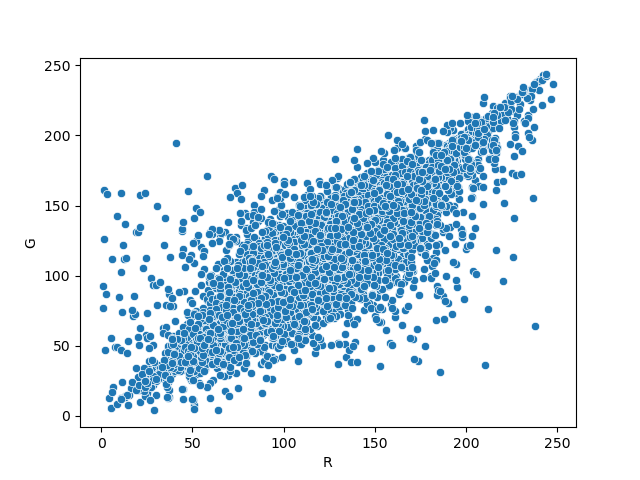
\includegraphics[width=1.0\textwidth]{scatter_r_g.png}
		\label{Fig.17}
	\end{figure}

	\begin{figure}[htbp]
		\centering
		\caption{特征$Gr$与特征$S$之间的散点图}
		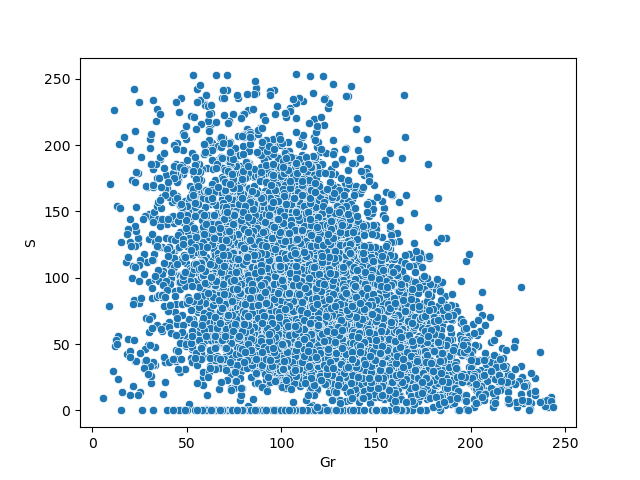
\includegraphics[width=1.0\textwidth]{scatter_gr_s.png}
		\label{Fig.18}
	\end{figure}

	为了更全面的展示特征两两之间的关系,我们在\hyperref[Fig.19]{图19}中绘制了七组特征两两之间的散点图。该图中对角线上为单个特征的直方图,非对角线上为特征两两之间的散点图。从图中可以看出:
	\begin{itemize}
		\item 特征$Gr$和$G$之间存在显著的正相关关系。
		\item 特征$R$和$G$之间,以及特征$G$和$B$之间存在着较为显著的正相关关系。
		\item 特征$Gr$与$S$之间,特征$G$与$S$之间,以及特征$B$与$S$之间存在着一定的负相关关系。
		\item 其他的特征之间,如$H$和$Gr$之间存在很弱的相关关系,或者不存在相关关系。
	\end{itemize} 
	
	\begin{figure}[htbp]
		\centering
		\caption{七组特征两两之间的散点图}
		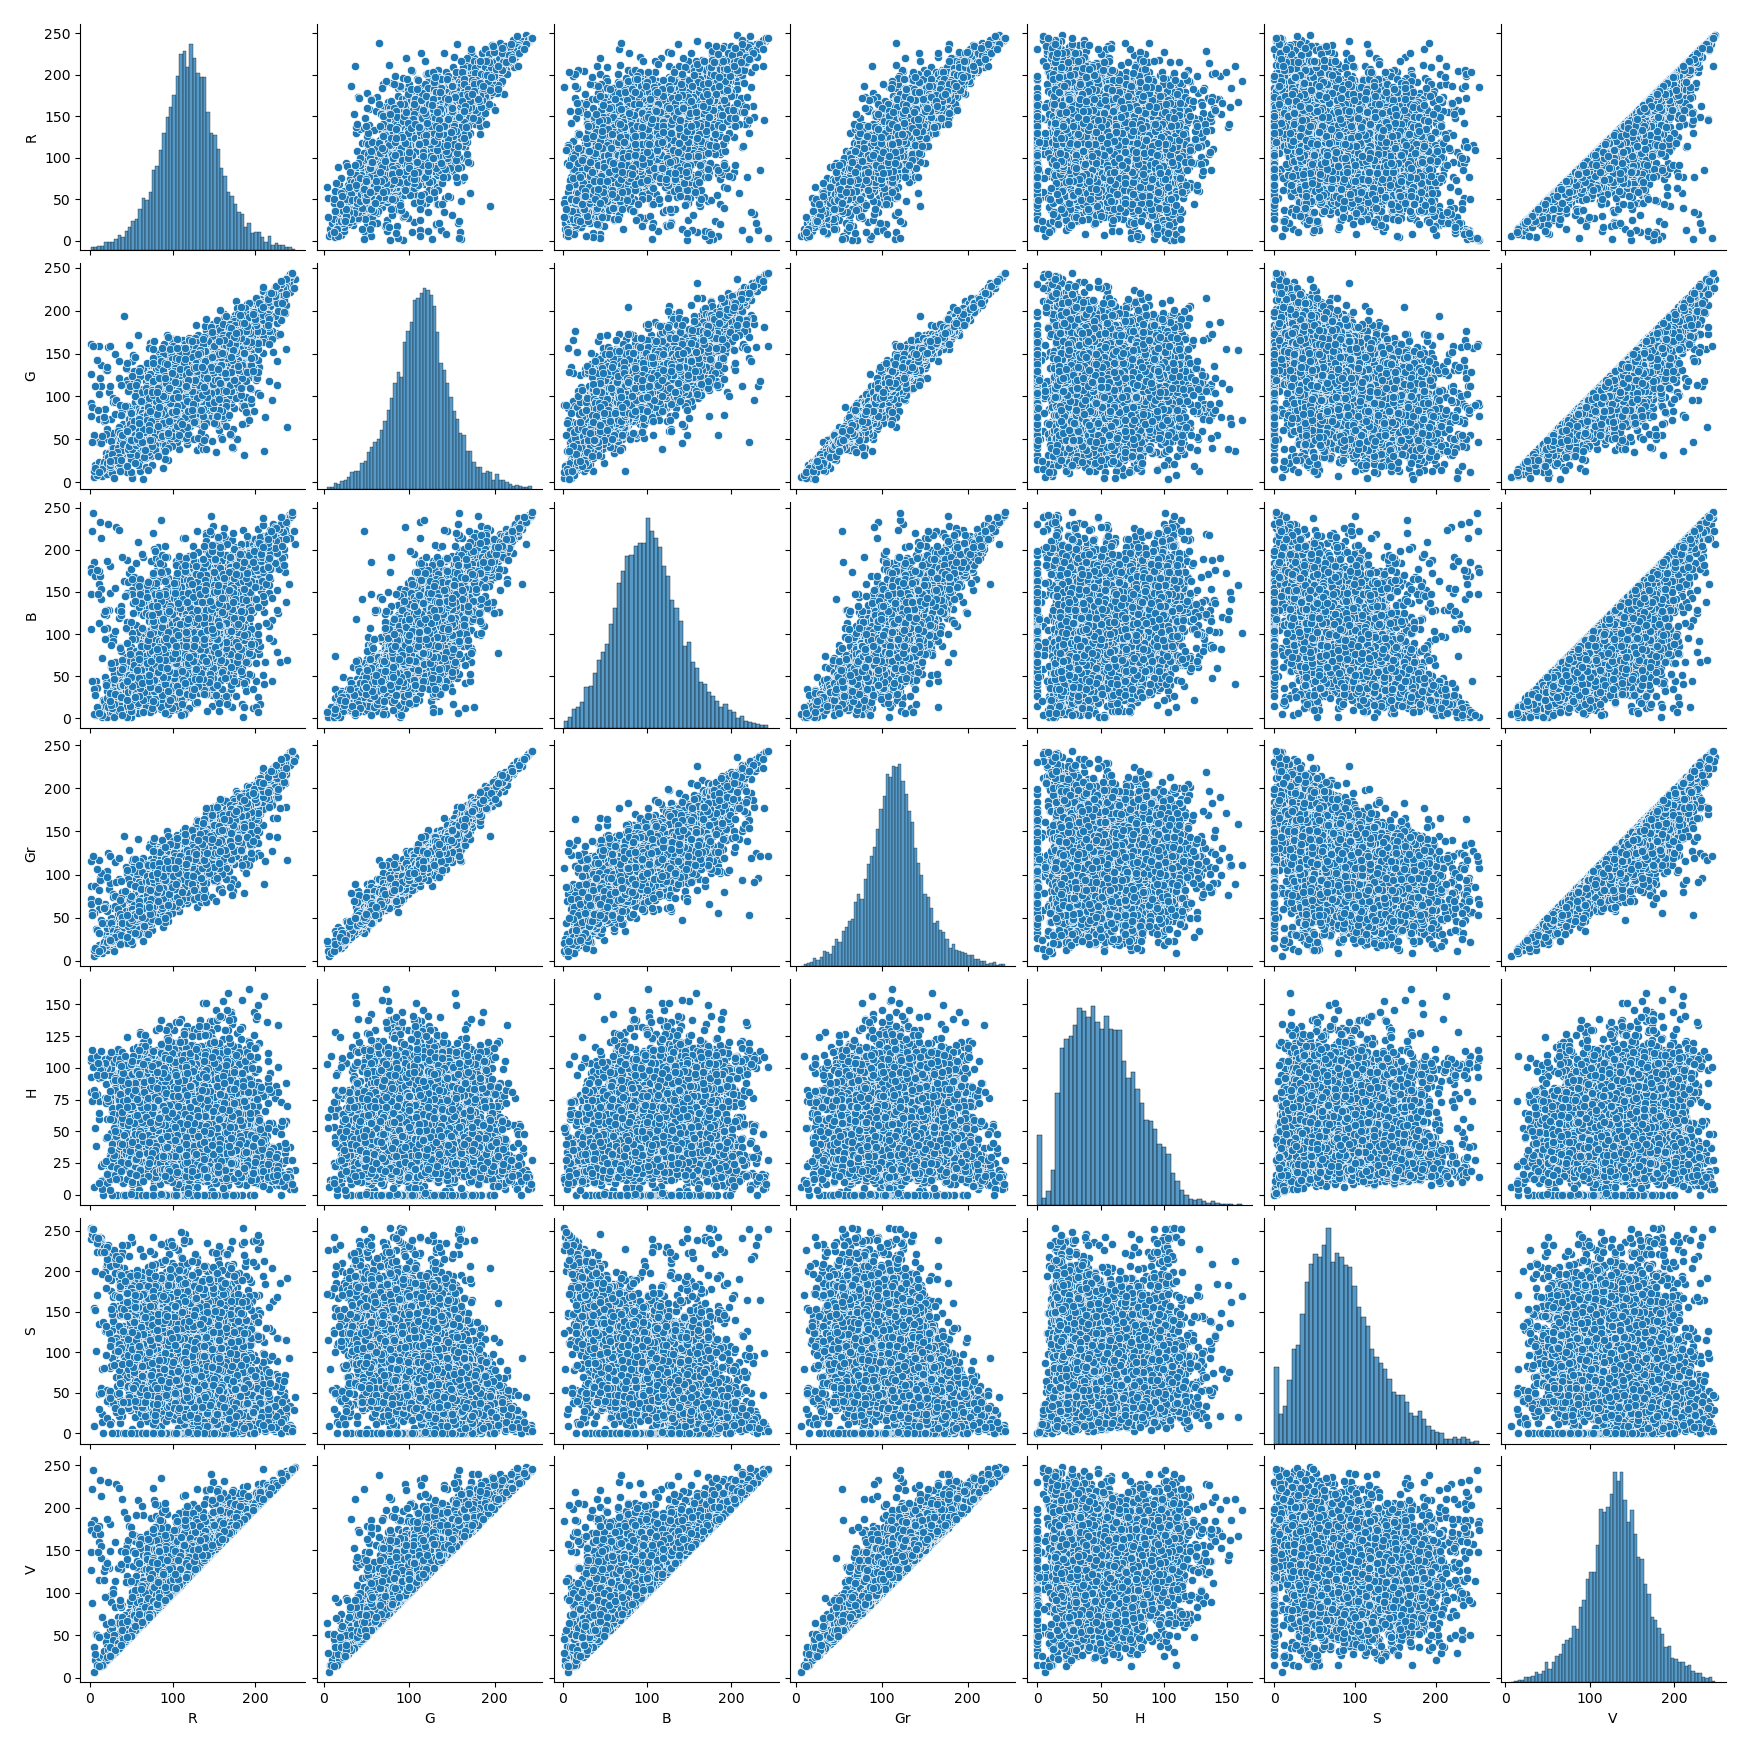
\includegraphics[width=1.0\textwidth]{pair_plot.png}
		\label{Fig.19}
	\end{figure}

	\subsubsection{折线图}
	使用折线图可以突出因变量随自变量的变化趋势。如\hyperref[Fig.20]{图20}中所示,我们绘制了特征$G$与特征$Gr$之间的折线图。可见特征$G$与特征$Gr$之间总体上呈正相关性。
	
	此外由于数据点过多($n=10000$),为了更好的展示效果,我们将特征$G$的数据中两两相差小于$1$的数据合并到一个点,并使用$95\%$的置信区间表示合并后的特征$G$对应的特征$Gr$的取值范围,如\hyperref[Fig.21]{图21}所示,其中阴影部分代表置信区间。从这张图中可以更明显地观察到特征$G$与特征$Gr$之间的正相关性。
	
	\begin{figure}[htbp]
		\centering
		\caption{特征$G$与特征$Gr$之间的折线图}
		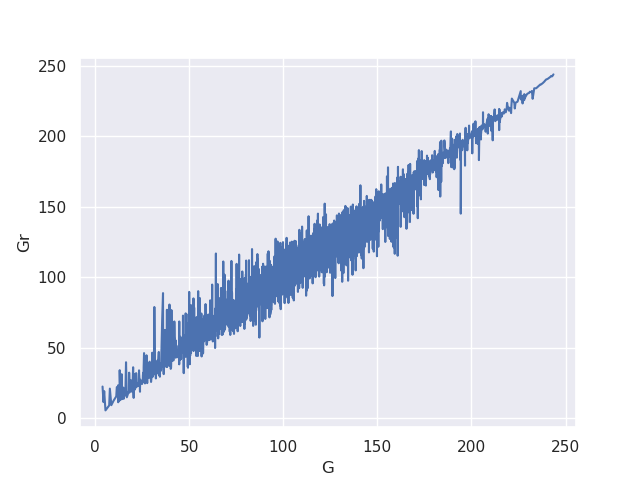
\includegraphics[width=1.0\textwidth]{line_g_gr.png}
		\label{Fig.20}
	\end{figure}

	\begin{figure}[htbp]
	\centering
	\caption{特征$G$与特征$Gr$之间的折线图}
	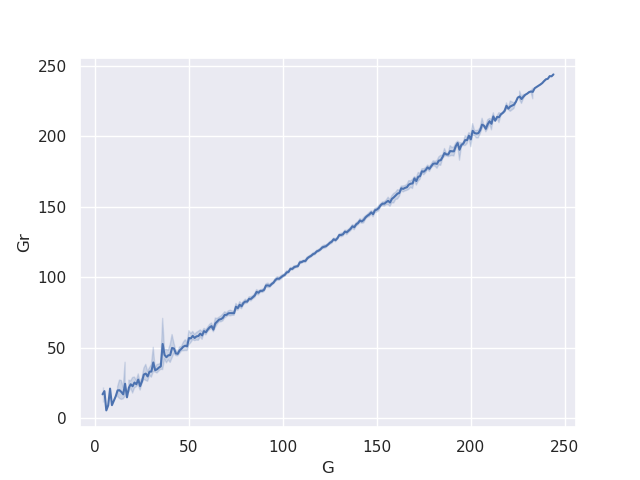
\includegraphics[width=1.0\textwidth]{line_g_gr_round.png}
	\label{Fig.21}
	\end{figure}
	
	为了方便综合比较,我们制作复合折线图,将多个其他特征的与$Gr$之间的关系放在一张图中进行比较。如\hyperref[Fig.22]{图22}和\hyperref[Fig.23]{图23}所示。其中\hyperref[Fig.22]{图22}展示了特征$R$,$G$,$B$分别与特征$Gr$之间的折线图,可见$R$,$G$,$B$三个特征与$Gr$之间都存在着较强的正相关性。\hyperref[Fig.23]{图23}展示了特征$H$,$S$,$V$分别与特征$Gr$之间的折线图,可见特征$V$与$Gr$之间存在较强的相关性,特征$S$与$Gr$之间存在较弱的负相关性,特征$H$与特征$Gr$之间相关性很弱。
	
	\begin{figure}[htbp]
		\centering
		\caption{特征$R$,$G$,$B$分别与特征$Gr$之间的折线图}
		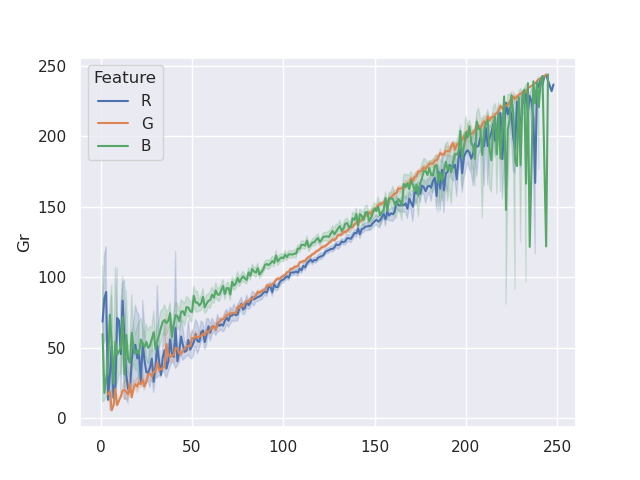
\includegraphics[width=1.0\textwidth]{line_r_g_b_gr_round.png}
		\label{Fig.22}
	\end{figure}
	
	\begin{figure}[htbp]
		\centering
		\caption{特征$H$,$S$,$V$分别与特征$Gr$之间的折线图}
		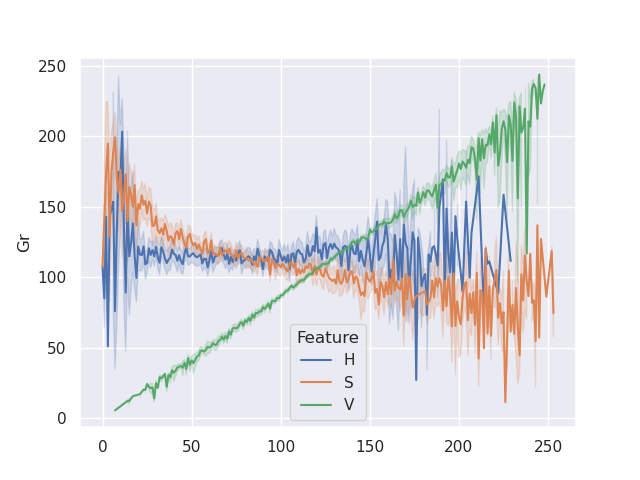
\includegraphics[width=1.0\textwidth]{line_h_s_v_gr_round.png}
		\label{Fig.23}
	\end{figure}

	\subsubsection{条形图}
	条形图使用等宽直条的长短表示各个相互独立的指标的大小,便于我们比较各个指标之间的差距。在数据的预处理和统计分析这一章中我们已经使用过直方图形式的条形图来展示各个特征的分布情况。在本小节中,我们进一步制作复合条形图,以便于更直观地比较各个特征的分布情况。
	
	在\hyperref[Fig.24]{图24}中我们绘制了特征$R$,$G$,$B$分布的复合条形图,从图中可以看出特征$R$和$G$在分布上非常接近,而特征$B$相比于其他两个特征偏度更大,也即呈右偏分布,峰度更小,也即呈扁平分布。这一结论和我们在\hyperref[Chart.11]{表11}中关于偏度峰度的计算结果形成了相互验证。
	
	在\hyperref[Fig.25]{图25}中我们绘制了特征$H$,$S$,$V$分布的复合条形图,从图中可以看出三个之间存在着显著的差别。在偏度上特征$S$最大,特征$H$次之,特征$V$最小。在峰度上特征$V$最大,特征$S$次之,特征$H$最小。这一结论和我们在\hyperref[Chart.11]{表11}中关于偏度峰度的计算结果形成了相互验证。
	
	\begin{figure}[htbp]
		\centering
		\caption{特征$R$,$G$,$B$分布的复合条形图}
		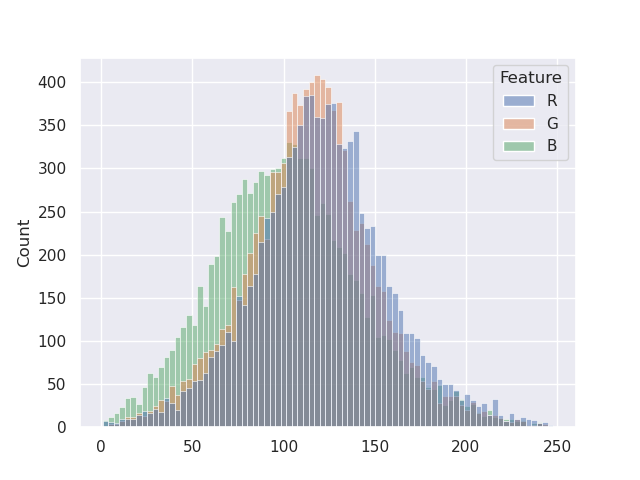
\includegraphics[width=1.0\textwidth]{hist_r_g_b.png}
		\label{Fig.24}
	\end{figure}
	
	\begin{figure}[htbp]
		\centering
		\caption{特征$H$,$S$,$V$分布的复合条形图}
		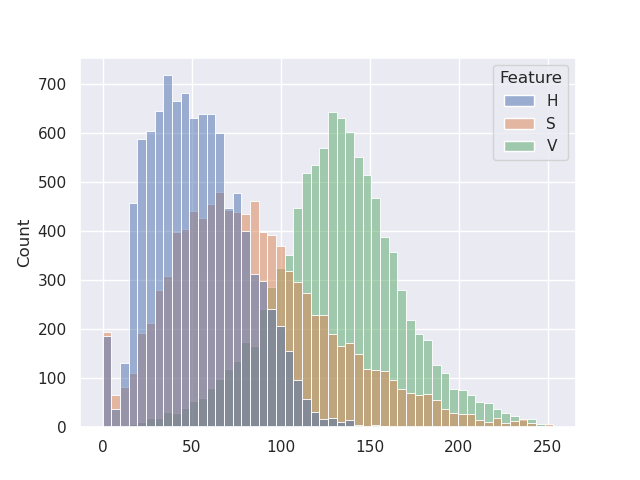
\includegraphics[width=1.0\textwidth]{hist_h_s_v.png}
		\label{Fig.25}
	\end{figure}
	
	\subsubsection{饼图}
	饼图可以反映单一指标的构成等信息。在饼图的基础上,环状饼图可以用不同的圆环表示不同的数据序列,从而弥补普通饼图在展示多属性上的不足。
	
	如\hyperref[Fig.26]{图26}所示,我们绘制了七组特征中各自异常数据所占比例的环状饼图,其中异常数据的判定使用的是统计检验之离群值检验这一小节中的拉伊达准则,具体判定标准见\hyperref[Chart.13]{表13}。该图中橙红色的区域代表离群值占总样本数的比例,其他颜色的区域代表各个特征的正常值占总样本数的比例。由外而内七个圆环依次代表特征$R$,$G$,$B$,$Gr$,$H$,$S$和$V$。
	
	从图中可以看出七组特征中离群值的占比都小于$1\%$。且离群值最少的是特征$B$,$H$和$V$,离群值占比仅为$0.4\%$。离群值最多的是特征$S$,离群值占比达$0.7\%$。
	
	\begin{figure}[htbp]
		\centering
		\caption{七组特征中各自离群值所占比例的环状饼图}
		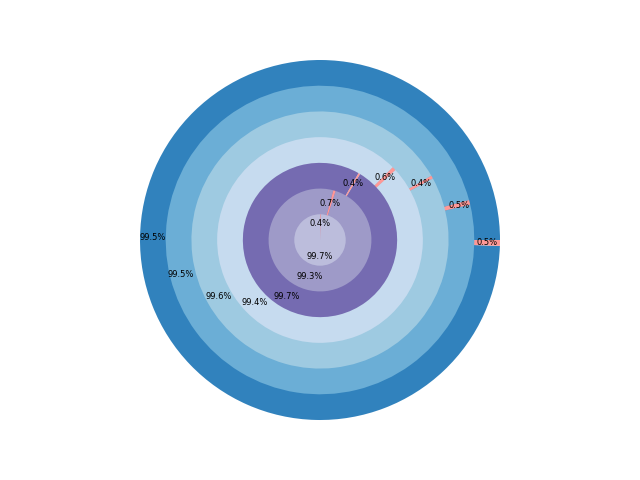
\includegraphics[width=1.0\textwidth]{pie.png}
		\label{Fig.26}
	\end{figure}
	
	\subsubsection{数据的图示实验总结}
	在数据的图示这一章中,我们分别使用了散点图,折线图,条形图和饼图进行了数据的可视化并进行了分析与对比。
	
	我们通过绘制七组特征两两之间的散点图,可视化了特征之间的相关性关系。发现了多组特征之间存在正相关关系,少数特征之间存在负相关关系,以及部分特征之间相关性很弱或者不存在相关性关系。
	
	我们通过在同一张图上绘制多组特征两两之间的折线图,更直观地观察到了特征之间的相关关系。
	
	我们通过在同一张图上绘制多组特征分布情况的条形图,对比了多组特征在分布上的相似情况。我们也根据绘图结果定性地判断了多个特征之间的偏度与峰度的大小关系,并和前文实验中计算得到的偏度峰度大小关系进行了对比与验证。
	
	最后我们通过绘制环状饼图,可视化了七组特征中各自的离群值占总样本数的比例。我们观察到所有特征的离群值占比都较少,且不同特征的离群值占比之间有着较大差异,最小占比仅为$0.4\%$,而最大占比为$0.7\%$。
	
	
	\section{数据的处理作业一}
	
	\subsection{作业要求}
	
		\begin{itemize}
		\item 结合实验室具体研究问题
		\item 样本数不得少于30个
		\item 样本数据的变量数不得少于三种
		\item 选取回归分析 OR 相关分析中的一种
		\begin{enumerate}
			\item 回归分析
			\begin{itemize}
				\item 开展两变量间的回归分析(可以是线性、非线性,logistic均可),并给出显著性检验
				\item 开展至少三变量之间的多元回归分析,并给出复相关系数和偏回归系数的显著性检验
				\item 对回归分析结果结合具体研究问题展开讨论
			\end{itemize} 
			\item 相关分析
			\begin{itemize}
				\item 根据其中两个变量的类型选定相关计算方法
				\item 计算相关系数,并做显著性检验
				\item 根据变量含义对各变量分组,
				\item 计算两组之间的典型相关系数
				\item 对相关分析结果结合具体研究问题展开讨论
			\end{itemize} 
		\end{enumerate}
		
	\end{itemize} 

	\subsection{实验介绍}
	在这一章中我们采用与数据的预处理和统计分析这一章中相同的数据进行实验。也即我们从ImageNet数据集中随机选择了10000张图片做为实验数据。对于每张图片,通过图像处理可以获得\hyperref[Chart.9]{表9}中的7项特征。因此总体的实验数据为$10000 \times 7$的矩阵,部分特征数据如\hyperref[Fig.8]{图8}所示。
	
	\subsection{回归分析}
	
	\subsubsection{两变量线性回归}
	
	\paragraph{回归问题} 我们选择特征$G$和特征$Gr$进行两变量的线性回归分析,每个特征包含$10000$条数据。特征$G$和特征$Gr$的之间散点图如\hyperref[Fig.27]{图27}所示,可见两个特征之间有较为显著的正相关关系。
	
	\begin{figure}[htbp]
		\centering
		\caption{特征$G$和特征$Gr$的之间散点图}
		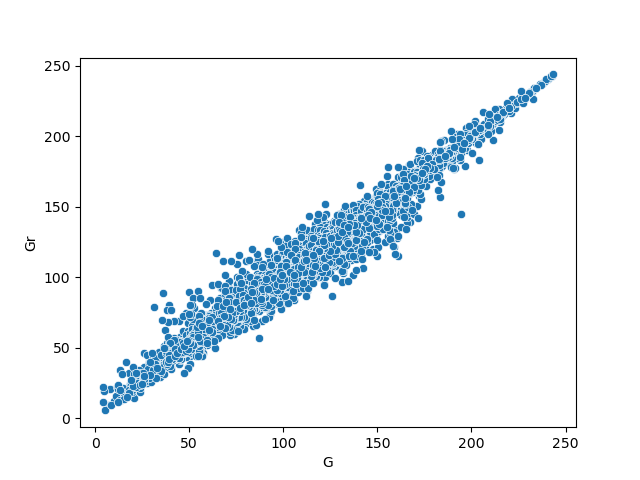
\includegraphics[width=1.0\textwidth]{scatter_g_gr.png}
		\label{Fig.27}
	\end{figure}

	\paragraph{回归方法} 设要求解的回归方程为$y = a + bx$,其中$a$和$b$是要求解的系数。我们可以使用最小二乘法求解使得误差
	\begin{equation*}
	Q(\hat{a}, \hat{b}) = \sum\limits_{i=1}^{n}[y_i - (a + bx_i)]^2
	\end{equation*}
	
	最小的系数$a$和$b$。等价于求解如下方程组
	\begin{align*}
	& na + b\sum\limits_{i=1}^{n}x_i = \sum\limits_{i=1}^{n}y_i \\
	& a\sum\limits_{i=1}^{n}x_i + b\sum\limits_{i=1}^{n}x_i^2 = \sum\limits_{i=1}^{n}x_iy_i
	\end{align*}
	
	求解过程为
	\begin{align*}
	& L_{xx} = \sum\limits_{i=1}^{n}(x_i - \bar{x})^2 = \sum\limits_{i=1}^{n}x_i^2 - \frac{1}{n}(\sum\limits_{i=1}^{n}x_i)^2 \\
	& L_{yy} = \sum\limits_{i=1}^{n}(y_i - \bar{y})^2 = \sum\limits_{i=1}^{n}y_i^2 - \frac{1}{n}(\sum\limits_{i=1}^{n}y_i)^2 \\
	& L_{xy} = \sum\limits_{i=1}^{n}(x_i - \bar{x})(y_i - \bar{y}) = \sum\limits_{i=1}^{n}x_iy_i - \frac{1}{n}(\sum\limits_{i=1}^{n}x_i)(\sum\limits_{i=1}^{n}y_i) \\
	& a = \bar{y} - b\bar{x}, \quad b = \frac{L_{xy}}{L_{xx}}
	\end{align*}
	
	此外我们可以通过决定系数:
	\begin{equation*}
	\frac{\sum\limits_{i=1}^{n}(\hat{y} - \bar{y})^2}{\sum\limits_{i=1}^{n}(y - \bar{y})^2}
	\end{equation*}
	
	来判断回归方程估测可靠程度的高低。
	
	\paragraph{回归结果} 按照公式求解可得
	\begin{align*}
	& a = \bar{y} - b\bar{x} = 5.2471 , \quad b = \frac{L_{xy}}{L_{xx}} = 0.9573
	\end{align*}
	
	也即求解得到的线性回归方程为
	\begin{equation*}
	y = a + bx = 5.2471 + 0.9573x
	\end{equation*}
	
	决定系数为:
	\begin{equation*}
	\frac{\sum\limits_{i=1}^{n}(\hat{y} - \bar{y})^2}{\sum\limits_{i=1}^{n}(y - \bar{y})^2} = 0.9685
	\end{equation*}
	
	我们将该线性回归方程绘制到特征$G$和特征$Gr$的散点图上,如\hyperref[Fig.28]{图28}所示,可见拟合效果是比较理想的。
	
	\begin{figure}[htbp]
		\centering
		\caption{特征$G$和特征$Gr$的线性回归方程}
		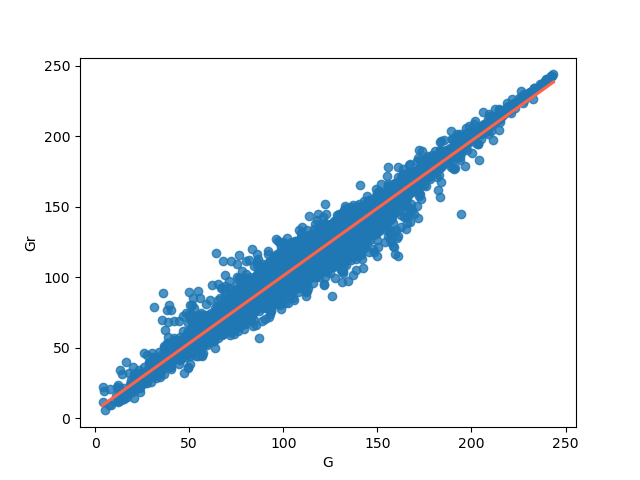
\includegraphics[width=1.0\textwidth]{scatter_g_gr_line.png}
		\label{Fig.28}
	\end{figure}

	\subsubsection{两变量线性显著性检验}
	
	\paragraph{检验问题} 求得回归方程只是完成了统计分析中两变量关系的统计描述,我们还需要回答它所来自的总体的直线回归关系是否确实存在。
	
	\paragraph{检验方法} 使用F检验:
	\begin{equation*}
	F = \frac{\frac{Q_x}{f_x}}{\frac{Q_e}{f_e}} = \frac{\frac{Q_x}{1}}{\frac{Q_e}{N-2}}
	\end{equation*}
	
	根据显著性水平$\alpha$比较计算得到的F值和$F_{\alpha}(1, N - 2)$的大小关系。若$F > F_{\alpha}(1, N - 2)$,则在显著性水平$\alpha$下,求解得到回归方程是显著的。
	
	\paragraph{检验结果} 首先计算回归平方和$Q_x$:
	\begin{equation*}
	Q_x = SS_r = \sum\limits_{i=1}^{n}(\hat{y} - \bar{y})^2 = 11482621.9177
	\end{equation*}
	
	再计算残差平方和$Q_e$:
	\begin{equation*}
	Q_e = SS_e = \sum\limits_{i=1}^{n}(y - \hat{y})^2 = 373415.2436
	\end{equation*}
	
	进而可以计算$F$:
	\begin{equation*}
	F = \frac{\frac{Q_x}{1}}{\frac{Q_e}{N-2}} = 307441.2625
	\end{equation*}
	
	取显著性水平$\alpha=0.01$,查表可知$F_{0.01}(1, 9998) < F_{0.01}(1, 600)=6.677$,因此$F > F_{0.01}(1, 9998)$。所以显著性检验的结论为在$0.01$水平上显著,也即可信赖程度在$99\%$以上。
	
	\subsubsection{两变量线性回归结果讨论}
	特征$G$和特征$Gr$之间存在很强的正相关性,在数据的预处理和统计分析这一章中,我们已经发现了这一结论。在线性回归这一小节,我们通过求解线性回归方程并进行显著性检验再次验证了这一结论。实际上从物理意义上来看,特征$Gr$代表图像的灰度,特征$G$代表图像在$RGB$色彩空间中的$G$分量,特征$Gr$是可以通过特征$R$,$G$,$B$线性组合得到的,因此特征$G$和特征$Gr$之间存在很强的正相关性也是合乎逻辑的。
	
	\subsubsection{多元线性回归}
	
	\paragraph{回归问题} 我们选择特征$H$,$S$,$V$作为自变量,特征$Gr$作为因变量进行多元线性回归分析,每个特征包含$10000$条数据。
	
	\paragraph{回归方法} 和两变量线性回归类似的,我们仍然通过最小二乘法求解残差平方和最小时的回归系数。设要求解的回归方程为:
	\begin{equation*}
	Y_i = \beta_1 + \beta_2X_{2i} + \beta_3X_{3i} + \cdots + \beta_kX_{ki} + \mu_i
	\end{equation*}
	
	其中$\beta_i$和$\mu_i$是要求解的系数。在矩阵形式下,多元线性回归方程可以表示为
	\begin{equation*}
	Y = X\beta + e
	\end{equation*}
	
	等式两边同时左乘$X'$
	\begin{equation*}
	X'Y = X'X\beta + X'e
	\end{equation*}
	
	根据最小二乘原则
	\begin{equation*}
	X'e = 0
	\end{equation*}
	
	则正规方程为
	\begin{equation*}
	X'X\hat{\beta} = X'Y
	\end{equation*}
	
	多元回归的普通最小二乘法估计量为
	\begin{equation*}
	\hat{\beta} = (X'X)^{-1}X'Y
	\end{equation*}
	
	此外我们可以通过计算复相关系数:
	\begin{equation*}
	R = \sqrt{\frac{Q_x}{Q_T}} = \sqrt{\frac{\sum\limits_{i=1}^{n}(\hat{y_i} - \bar{y})^2}{\sum\limits_{i=1}^{n}(y_i - \bar{y_i})^2}}
	\end{equation*}
	
	来判断因变量和多个自变量之间的线性相关程度。
	
	\paragraph{回归结果} 根据回归公式计算可得
	\begin{align*}
	& \hat{\beta} = [-0.1060, -0.2197, 0.8604]\\
	& \mu = 25.8570
	\end{align*}
	
	也即求解得到的多元线性回归方程为
	\begin{equation*}
	y = \hat{\beta}\hat{x} + \mu = -0.1060x_1 - -0.2197x_2 + 0.8604x_3 + 25.8570
	\end{equation*}
	
	复相关系数为:
	\begin{equation*}
	R = \sqrt{\frac{\sum\limits_{i=1}^{n}(\hat{y_i} - \bar{y})^2}{\sum\limits_{i=1}^{n}(y_i - \bar{y_i})^2}} = 0.9785
	\end{equation*}
	
	其值说明特征$Gr$与特征$H$,$S$,$V$之间存在较强的线性相关关系。
	
	\subsubsection{多元线性回归显著性检验}
	
	\paragraph{检验问题} 和两变量线性回归类似的,我们需要检验多元线性回归方程是否显著。
	
	\paragraph{检验方法} 首先我们需要检验所有自变量联合起来对因变量影响的显著性,需要在方差分析的基础上进行F检验。原假设:
	\begin{equation*}
	H_0: \beta_2 = \beta_3 = \cdots = \beta_k = 0
	\end{equation*}
	
	也即所有解释变量联合起来时对被解释变量的影响不显著。备择假设:
	\begin{equation*}
	H_1: \beta_j \neq 0 \ for \ some \   j=1,2,\cdots,k
	\end{equation*}
	
	建立统计量:
	\begin{equation*}
	F = \frac{\frac{Q_x}{k - 1}}{\frac{Q_e}{n - k}} = \frac{\frac{\sum\limits_{i=1}^{n}(\hat{y_i} - \bar{y})^2}{k-1}}{\frac{\sum\limits_{i=1}^{n}(y_i - \bar{y})^2}{n-k}} \sim F(k-1, n-k)
	\end{equation*}
	
	根据显著性水平$\alpha$比较计算得到的F值和$F_{\alpha}(k-1, n-k)$的大小关系。若$F > F_{\alpha}(k-1, n-k)$,则在显著性水平$\alpha$下,求解得到回归方程是显著的。
	
	由于在但多元回归中,F检验显著不代表每个自变量都对$Y$有显著影响,因此还需要分别检验当其他自变量保持不变时,各个自变量对因变量是否有显著影响。首先需要计算偏回归系数$\beta_j$的标准化回归系数$P_j$:
	\begin{equation*}
	P_j= |\beta_j|\sqrt{\frac{L_{jj}}{Q_T}}
	\end{equation*}
	
	其中,$L_{jj}$为$X_j$的离差平方和,$Q_T$为$Y$的离差平方和。$P_j$越大,则对应的因素$X_j$越重要。
	
	对偏回归系数做显著性检验,我们需要计算每个偏回归系数的偏回归平方和:
	\begin{align*}
	& F_j = \frac{U_j}{\frac{Q_e}{n - k}}\\
	& U_j = \sum\limits_{i=1}^{n}(\beta_j(x_ji - \bar{x_j}))^2
	\end{align*}
	
	如果$F < F_{\alpha}(1, n - k)$,则说明$x_i$对$y$的影响是不显著的,可以将它从回归方程中去掉。
	
	\paragraph{检验结果} 首先检验所有自变量联合起来对因变量影响的显著性,计算回归平方和$Q_x$:
	\begin{equation*}
	Q_x = SS_r = \sum\limits_{i=1}^{n}(\hat{y} - \bar{y})^2 = 11351202.6208
	\end{equation*}
	
	再计算残差平方和$Q_e$:
	\begin{equation*}
	Q_e = SS_e = \sum\limits_{i=1}^{n}(y - \hat{y})^2 = 504834.5405
	\end{equation*}
	
	进而可以计算$F$:
	\begin{equation*}
	F = \frac{\frac{\sum\limits_{i=1}^{n}(\hat{y_i} - \bar{y})^2}{k-1}}{\frac{\sum\limits_{i=1}^{n}(y_i - \bar{y})^2}{n-k}} = 74920.0067
	\end{equation*}
	
	取显著性水平$\alpha=0.01$,查表可知$F_{0.01}(3, 9996) < F_{0.01}(3, 600)=3.814$,因此$F > F_{0.01}(3, 9996)$。所以显著性检验的结论为所有自变量联合起来对因变量的影响在$0.01$水平上显著,也即可信赖程度在$99\%$以上。
	
	接下来我们计算偏回归系数$\beta_j$的标准化回归系数$P_j$:
	\begin{align*}
	& P_1= |\beta_1|\sqrt{\frac{L_{11}}{Q_T}} = 0.0813 \\
	& P_2= |\beta_2|\sqrt{\frac{L_{22}}{Q_T}} = 0.2874\\
	& P_3= |\beta_3|\sqrt{\frac{L_{33}}{Q_T}} = 0.9012
	\end{align*}
	
	从标准化回归系数$P_j$可知,三个特征中,$V$最重要,$S$其次,$H$最不重要。
	
	接下来对偏回归系数做显著性检验,计算每个偏回归系数的偏回归平方和:
	\begin{align*}
	& U_1 = \sum\limits_{i=1}^{n}(\beta_j(x_1i - \bar{x_1}))^2= 78364.9718 \\
	& U_2 = \sum\limits_{i=1}^{n}(\beta_j(x_2i - \bar{x_2}))^2= 979310.3152 \\
	& U_3 = \sum\limits_{i=1}^{n}(\beta_j(x_3i - \bar{x_3}))^2= 9630455.8956 \\
	& F_1 = \frac{U_1}{\frac{Q_e}{n - k}}= 1551.6693 \\
	& F_2 = \frac{U_2}{\frac{Q_e}{n - k}}= 19390.8798 \\
	& F_3 = \frac{U_3}{\frac{Q_e}{n - k}} = 190688.2937
	\end{align*}
	
	取显著性水平$\alpha=0.01$,查表可知$F_{0.01}(1, 9996) < F_{0.01}(1, 600)=6.677$,因此$F_1$,$F_2$,$F_3$均大于$F_{0.01}(1, 9996)$。所以显著性检验的结论为3个自变量分别对于因变量的影响在$0.01$水平上都显著,也即可信赖程度在$99\%$以上。
	
	\subsubsection{多元线性回归结果讨论}
	在多元线性回归的实验中,我们得到了自变量$H$,$S$,$V$关于因变量的$Gr$的多元线性回归方程,并通过显著性检验证明了3个变量总体上对于因变量的影响,以及3个变量单独对于因变量的影响都是显著的。实际上从物理意义上来看,特征$Gr$代表图像的灰度,特征$H$,$S$,$V$分别代表图像在$HSV$色彩空间中的三个分量。特征$Gr$是可以通过$RGB$色彩空间中的特征$R$,$G$,$B$线性组合得到的,而$HSV$色彩空间又可以通过$RGB$色彩空间转化得到,因此特征$H$,$S$,$V$和特征$Gr$之间存在着本小节所得到的多元线性回归方程是合乎逻辑的。

	\section{数据的处理作业二}
		
	\subsection{作业要求}
	
	\begin{itemize}
		\item 结合实验室具体研究问题
		\item 样本数不得少于30个
		\item 选取聚类分析 OR 降维分析中的一种
		\begin{enumerate}
			\item 聚类分析
			\begin{itemize}
				\item 样本数据的变量数不得少于两种
				\item 根据数据类型,选取相似性测度方法
				\item 选定聚类的目标类数
				\item 选定类间距离计算方式
				\item 选定聚类算法并给出聚类过程
				\item 对聚类结果进行分析
			\end{itemize} 
			\item 降维分析
			\begin{itemize}
				\item 样本数据的变量数不得少于四种
				\item 根据数据类型选择PCA或者LDA
				\item 给出降维分析中各主成分或者LDA特征
				\item 给出选择最终降维成分的依据
				\item 分析降维后新变量与原始变量之间关系
			\end{itemize} 
		\end{enumerate}
	
	\end{itemize} 

	\subsection{实验介绍}
	
	在这一章中我们采用与数据的预处理和统计分析这一章中相同的数据进行实验。也即我们从ImageNet数据集中随机选择了10000张图片做为实验数据。对于每张图片,通过图像处理可以获得\hyperref[Chart.9]{表9}中的7项特征。因此总体的实验数据为$10000 \times 7$的矩阵,部分特征数据如\hyperref[Fig.8]{图8}所示。
	
	\subsection{降维分析} 
	
	\subsubsection{降维问题} 
	
	PCA即主成分分析(Principal Component Analysis),是一种常用的降维方法。PCA可以在尽可能多地保留原始数据的信息的前提下,将大量的相关特征转化成少数的无关特征,这些少数的无关特征就是主成分。在本次实验中,我们使用PCA对具有7项特征的10000条数据进行降维。
	
	\subsubsection{降维方法}
	
	在PCA之前,我们首先要将数据进行标准化,也即使得特征的均值为0,方差为1:
	\begin{equation*}
	x_i' = \frac{x_i - \bar{x_i}}{\sqrt{D(x_i)}}
	\end{equation*}
	
	其中$x_i$代表原始的第$i$个特征,$\bar{x_i}$代表第$i$个特征的均值,$D(x_i)$代表第$i$个特征的方差,$x_i'$代表标准化后的第$i$个特征。
	
	设$X = (X_1, X_2, \cdots, X_p)$的协方差矩阵为$\sigma$,其特征根为
	\begin{equation*}
	\lambda_1 \geq \lambda_2 \geq \cdots \lambda_p \geq 0
	\end{equation*}
	
	相应的单位化的特征向量为
	\begin{equation*}
	T_1, T_2, \cdots, T_p
	\end{equation*}
	
	那么,由此确定的主成分为
	\begin{equation*}
	Y_1 = T_1'X, \ Y_2 = T_2'X, \ \cdots, \ Y_m = T_m'X
	\end{equation*}
	
	主成分的方差分别为$\sigma$的特征值
	\begin{equation*}
	\lambda_1, \lambda_2, \cdots \lambda_m
	\end{equation*}
	
	为了确定多少个主成分是足够的,我们可以计算累计贡献率:
	\begin{equation*}
	\frac{\sum\limits_{k=1}^{i} \lambda_k}{\sum\limits_{k=1}^{p} \lambda_k}, \quad i=1,2,\cdots, p
	\end{equation*}
	
	一般可以取累计贡献率达$85\sim 95\%$的特征值所对应的前$m(m \leq p)$个主成分。
	
	~\
	
	PCA降维的步骤可以总结为:
	\begin{itemize}
		\item 对数据做标准化
		\item 求特征协方差矩阵
		\item 求协方差矩阵的特征值和特征向量
		\item 将特征值按照从大到小的顺序排列,选择其中最大的$k$个,将其对应的$k$个特征向量分别作为列向量组成特征向量矩阵
		\item 将样本点投影到选取的特征向量上。这样,就将原始样例的$n$维特征变成了$k$维,这$k$维就是原始特征在$k$维上的投影,代表了原始的$n$个特征。
	\end{itemize} 

	\subsubsection{降维过程} 首先我们对具有7项特征的10000条数据进行标准化,部分标准化后的数据如\hyperref[Fig.29]{图29}和所\hyperref[Fig.30]{图30}所示。
	
	\begin{figure}[htbp]
		\centering
		\caption{第$1\sim20$条数据标准化后的结果}
		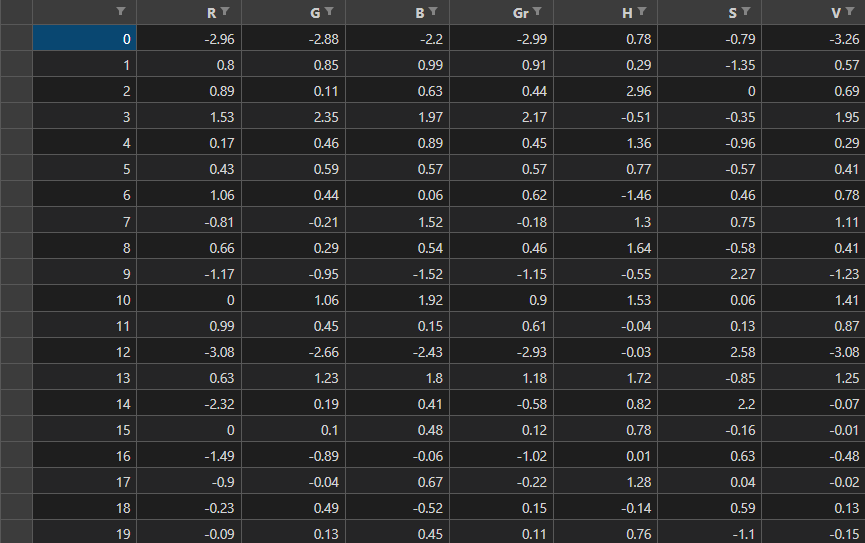
\includegraphics[width=1.0\textwidth]{data_standard1.png}
		\label{Fig.29}
	\end{figure}

	\begin{figure}[htbp]
		\centering
		\caption{第$9981\sim10000$条数据标准化后的结果}
		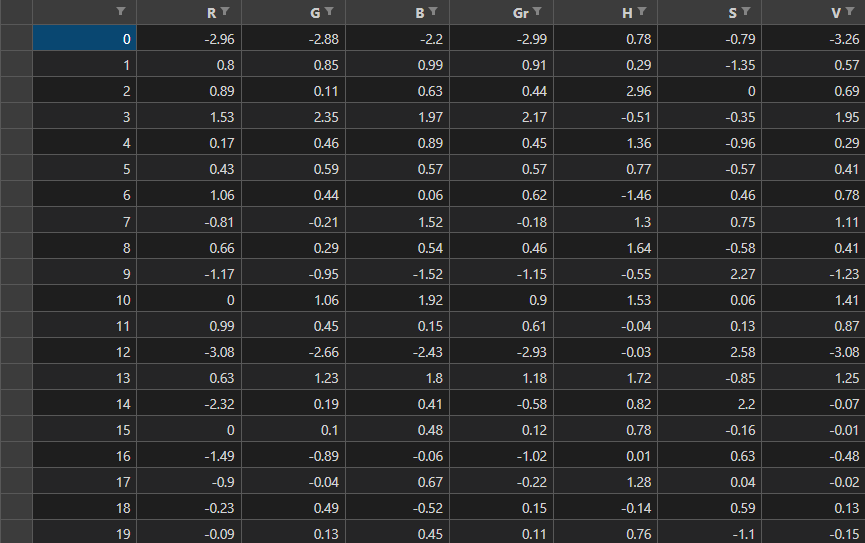
\includegraphics[width=1.0\textwidth]{data_standard1.png}
		\label{Fig.30}
	\end{figure}
	
	接着我们计算标准化后的特征的协方差矩阵:
	\begin{equation*}
	\Sigma = 
	\begin{bmatrix}
	1.0001 & 0.8286 & 0.6350 &  0.9070 &  -0.1525 &-0.2790  & 0.8814  \\
	0.8286 & 1.0001 & 0.8495 & 0.9842 & 0.0411& -0.3975 & 0.9029  \\
	0.6350  & 0.8495 & 1.0001 & 0.8514 & 0.3443& -0.5592 & 0.7957  \\ 
	0.9070  & 0.9842 & 0.8514 & 1.0001& 0.0221 &-0.4049 & 0.9353  \\
	-0.1525 & 0.0411 & 0.3443 & 0.0221 & 1.0001& -0.1124 & 0.0789  \\
	-0.279 & -0.3975 &-0.5592 &-0.4049 &-0.1124 & 1.0001& -0.1404  \\
	0.8814 & 0.9029 & 0.7957 & 0.9353 & 0.0789 &-0.1404 & 1.0001  \\
	\end{bmatrix}
	\end{equation*}
	
	对矩阵进行特征值分解后可以得到特征值从到大小为:
	\begin{equation*}
	\hat{\lambda} = 
	\begin{bmatrix}
	4.6201 & 1.2311 & 0.8624 & 0.1868 & 0.0840 & 0.0162 & 0.0000 \\
	\end{bmatrix}
	\end{equation*}
	
	\subsubsection{选择最终降维成分的依据} 上述的特征值同时也是主成分的方差。我们可以作出主成分累计贡献率折线图,如\hyperref[Fig.31]{图31}所示。可知当选择2个主成分时,累计贡献率为
	\begin{equation*}
	\frac{\sum\limits_{k=1}^{2} \lambda_k}{\sum\limits_{k=1}^{7} \lambda_k} = 0.8358
	\end{equation*}
	
	当选择3个主成分时,累计贡献率为
	\begin{equation*}
	\frac{\sum\limits_{k=1}^{3} \lambda_k}{\sum\limits_{k=1}^{7} \lambda_k} = 0.9590
	\end{equation*}
	
	因此我们选择使得累计贡献率超过$85\%$的最少的主成分个数,也即$3$个。
	
	
	\begin{figure}[htbp]
		\centering
		\caption{主成分累计贡献率折线图}
		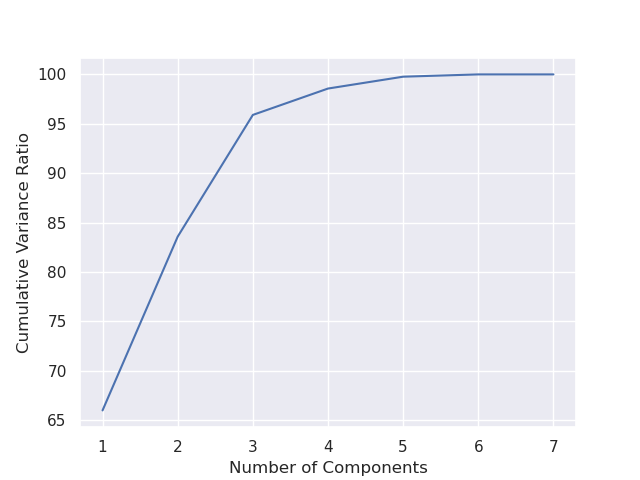
\includegraphics[width=1.0\textwidth]{pca_variance.png}
		\label{Fig.31}
	\end{figure}
	
	\subsubsection{降维后新变量与原始变量之间关系} 
	
	根据矩阵特征值分解的结果,我们选择了对应3个最大特征值的主成分,它们分别为
	\begin{align*}
	& x_1'=  0.4128x1 +  0.4509x2 + 0.4199x_3 + 0.4613x_4 + 0.0467x_5 - 0.2161x_6 + 0.4339x_7 \\
	& x_2' = 0.2980x1 +  0.0564x2 - 0.3045x_3 + 0.0889x_4 - 0.7830x_5 + 0.4148x_6 + 0.1489x_7 \\
	& x_3' = 0.0084x1 +  0.0182x2 - 0.0061x_3 + 0.0128x_4 + 0.4965x_5 + 0.8086x_6 + 0.3146x_7
	\end{align*}
	
	其中$x_1'$,$x_2'$和$x_3'$分别代表降维后的第一,第二和第三个特征。从新特征的表达式中我们可以观察到降维后的新变量与原始变量之间的关系:
	\begin{itemize}
		\item 在$x_1'$特征中,原第一、二、三、四、七特征,即特征$R$,$G$,$B$,$Gr$,$V$的系数都较大,这说明这些特征对于新特征$x_1'$的作用很大。而原第五特征,即特征$H$的系数很小,说明它对于新特征$x_1'$的作用很小。
		\item 在$x_2'$特征中,原第五特征,即特征$H$的系数很大,且显著大于其他六个特征,说明其对于新特征$x_2'$的作用很大。原第六特征,即特征$S$的系数较大,说明其对于新特征$x_2'$具有较大的作用。原第二、四特征,即特征$G$,$Gr$的系数很小,说明它们对于新特征$x_2'$的作用很小。
		\item 在$x_3'$特征中,原第六特征,即特征$S$的系数很大,且显著大于其他六个特征,说明其对于新特征$x_3'$的作用很大。原第五特征,即特征$H$的系数较大,说明其对于新特征$x_3'$具有较大的作用。原第一、二、三、四特征,即特征$R$,$G$,$B$,$Gr$的系数很小,说明它们对于新特征$x_3'$的作用很小。
	\end{itemize} 
	
	根据新特征与原始特征之间的表达式,我们可以将原来具有7项特征的10000条数据降维到仅有3项特征,且仍然保留了原始数据中$95.90\%$的信息。部分降维后的数据如\hyperref[Fig.32]{图32}和\hyperref[Fig.33]{图33}所示。
	
	\begin{figure}[htbp]
		\centering
		\caption{第$1\sim20$条数据降维后的结果}
		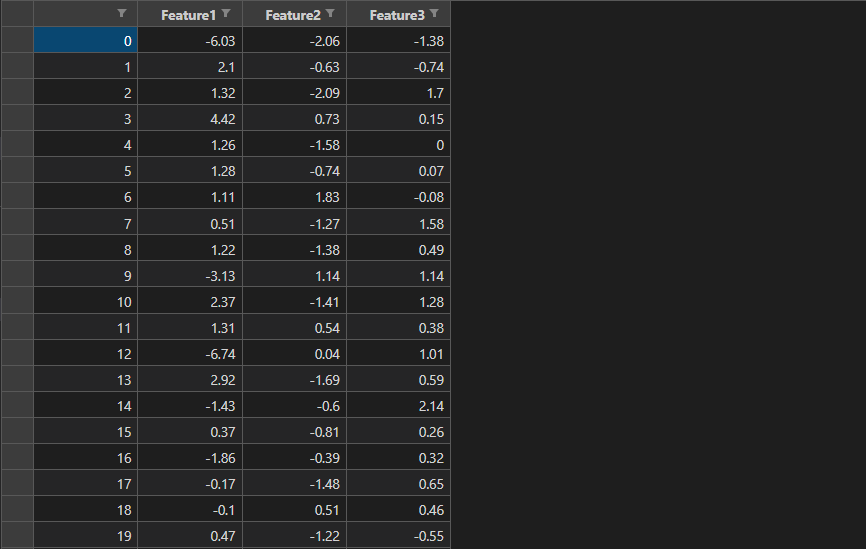
\includegraphics[width=1.0\textwidth]{data_pca1.png}
		\label{Fig.32}
	\end{figure}
	
	\begin{figure}[htbp]
		\centering
		\caption{第$9981\sim10000$条数据降维后的结果}
		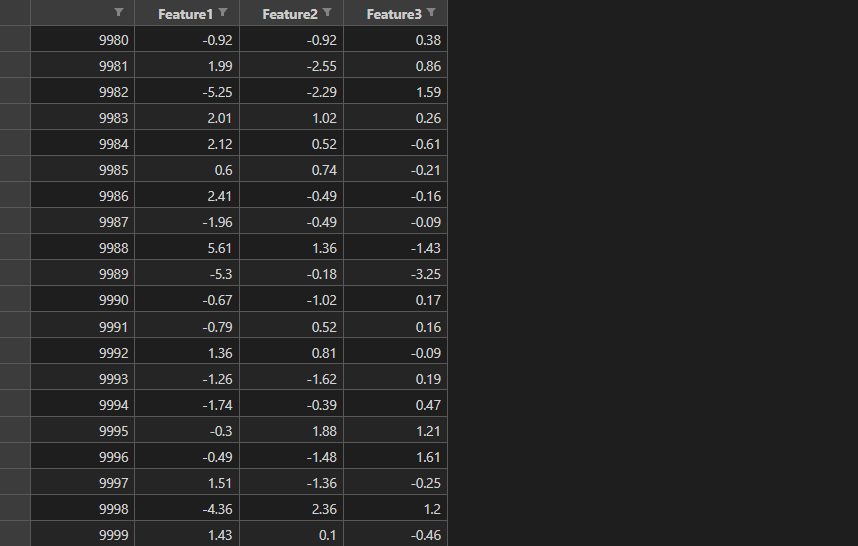
\includegraphics[width=1.0\textwidth]{data_pca2.png}
		\label{Fig.33}
	\end{figure}
	
	\subsection{聚类分析} 
	
	\subsubsection{聚类问题} 聚类属于无监督学习的一种,我们希望自动地将所有的样本划分为不同的类别。一个好的聚类结果,应该有高的簇内相似性和低的簇间相似性。
	
	\subsubsection{聚类方法} 在7项特征中,我们选择$V$和$S$这两项特征进行聚类分析。特征$V$和$S$之间的散点图如\hyperref[Fig.34]{图34}所示。
	
	\begin{figure}[htbp]
		\centering
		\caption{特征$V$和$S$之间的散点图}
		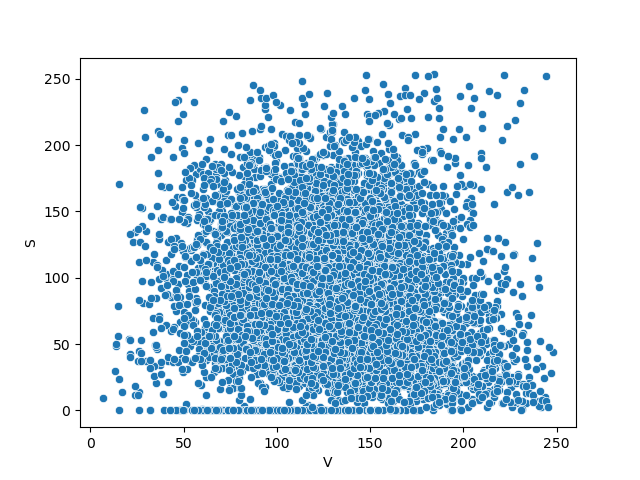
\includegraphics[width=1.0\textwidth]{scatter_v_s.png}
		\label{Fig.34}
	\end{figure}

	\paragraph{相似性测度} 在相似性测度上,我们选择欧式距离:
	\begin{equation*}
	d(\bar{x}, \bar{y}) = ||\bar{x} -  \bar{y}|| = [\sum\limits_{i=1}^n (x_i - y_i)^2]^{
	\frac{1}{2}}
	\end{equation*}
	
	\paragraph{聚类的目标类数} 在聚类的目标类数上,我们选择2,3,4类分别进行实验
	
	\paragraph{类间距离计算方式} 在类间距离计算方式上,我们使用平均距离:
	\begin{equation*}
	D_{pq}^2 = \frac{1}{n_pn_q} \sum_{x_i \in w_p, x_j \in w_q} d_{ij}^2
	\end{equation*}
	
	\paragraph{聚类算法} 在聚类算法上,我们选择K-Means算法,对于我们实验所用的大样本数据(样本数为10000),它具有实现方便且运算速度快的优点。K-Means算法的流程为:
	\begin{enumerate}
		\item 从$n$个数据对象任意选择$k$个对象作为初始聚类中心
		\item 对于待分类的数据点,根据其到各个聚类中心的欧式距离,将其划分到距离最小的簇
		\item 对于每一个簇,计算其内所有点的平均值作为新的聚类中心
		\item 如果聚类中心不再变化则聚类结束,否则返回第二步
	\end{enumerate}

	\subsubsection{聚类过程} 当聚类类别数为3时,聚类过程如\hyperref[Fig.35]{图35}至\hyperref[Fig.44]{图44}所示,聚类过程在10次迭代后满足终止条件。	
	
	\begin{figure}[htbp]
		\centering
		\caption{3类别数聚类,迭代次数为1时}
		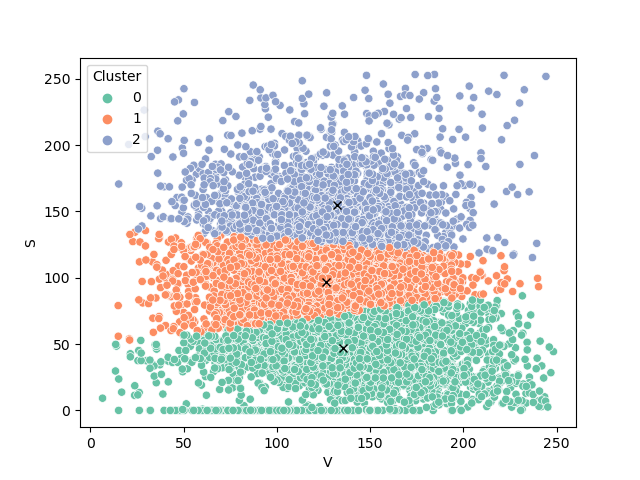
\includegraphics[width=1.0\textwidth]{cluster1.png}
		\label{Fig.35}
	\end{figure}
	
	\begin{figure}[htbp]
		\centering
		\caption{3类别数聚类,迭代次数为2时}
		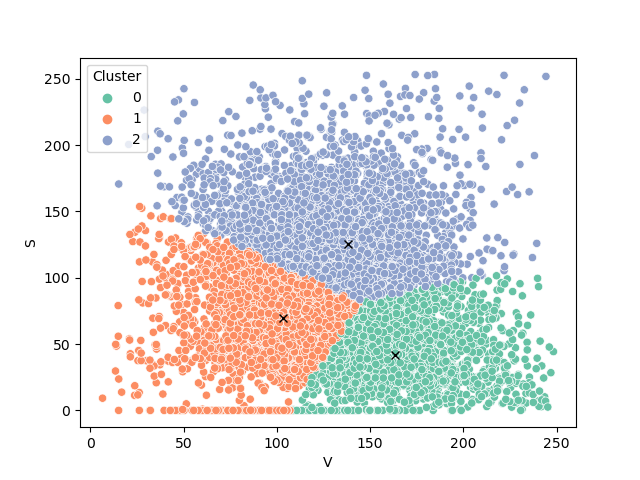
\includegraphics[width=1.0\textwidth]{cluster2.png}
		\label{Fig.36}
	\end{figure}
	
	\begin{figure}[htbp]
		\centering
		\caption{3类别数聚类,迭代次数为3时}
		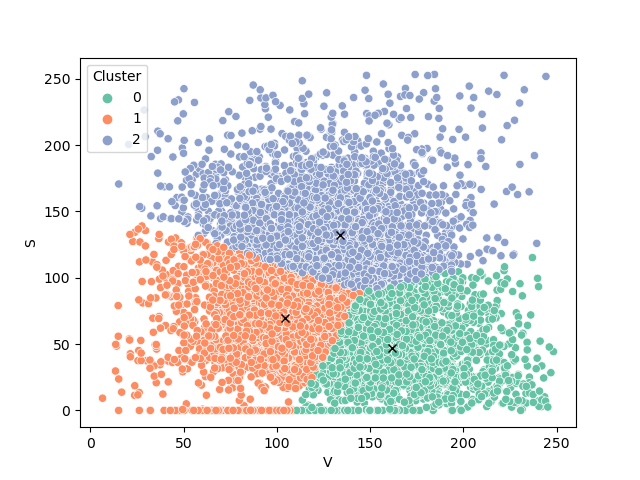
\includegraphics[width=1.0\textwidth]{cluster3.png}
		\label{Fig.37}
	\end{figure}

	\begin{figure}[htbp]
		\centering
		\caption{3类别数聚类,迭代次数为4时}
		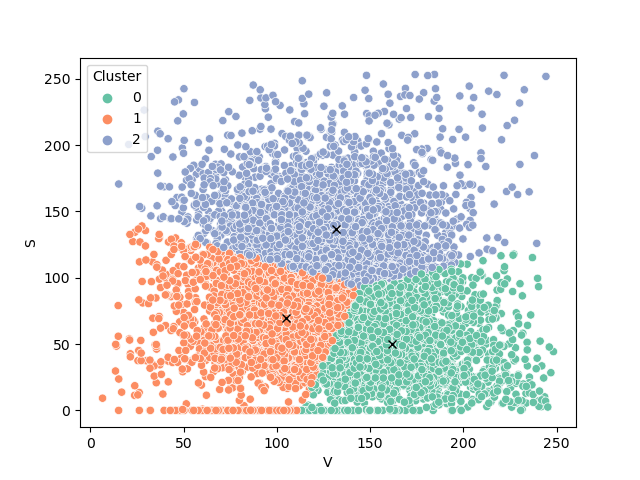
\includegraphics[width=1.0\textwidth]{cluster4.png}
		\label{Fig.38}
	\end{figure}

	\begin{figure}[htbp]
	\centering
	\caption{3类别数聚类,迭代次数为5时}
	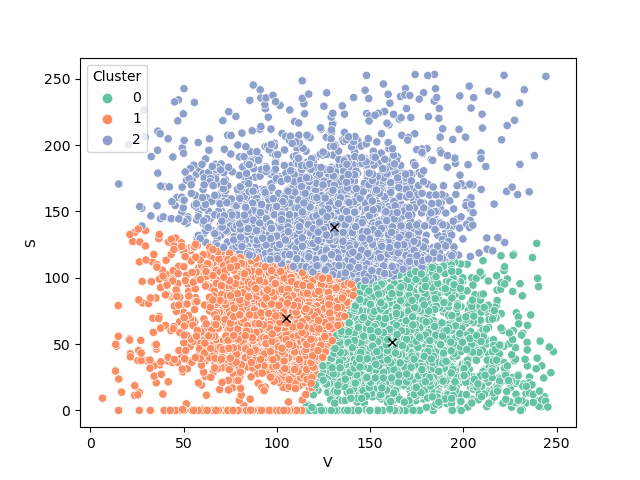
\includegraphics[width=1.0\textwidth]{cluster5.png}
	\label{Fig.39}
	\end{figure}

	\begin{figure}[htbp]
	\centering
	\caption{3类别数聚类,迭代次数为6时}
	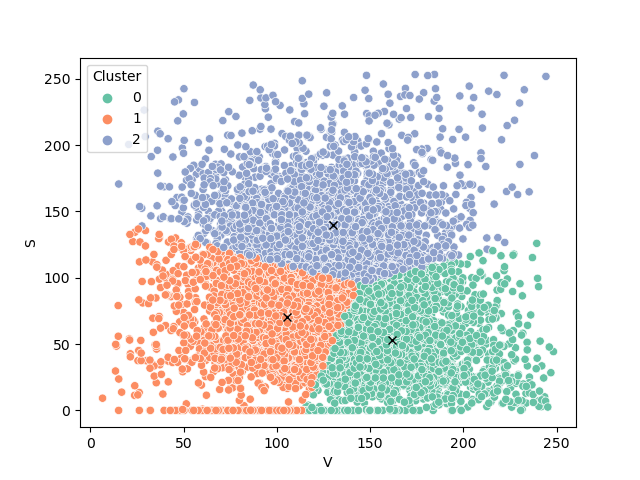
\includegraphics[width=1.0\textwidth]{cluster6.png}
	\label{Fig.40}
	\end{figure}

	\begin{figure}[htbp]
	\centering
	\caption{3类别数聚类,迭代次数为7时}
	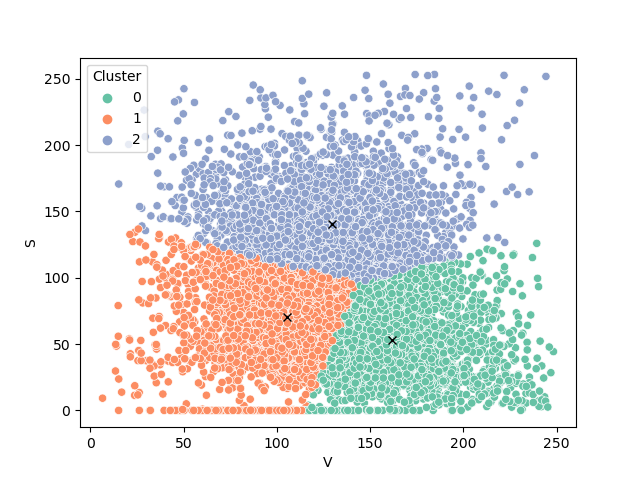
\includegraphics[width=1.0\textwidth]{cluster7.png}
	\label{Fig.41}
	\end{figure}

	\begin{figure}[htbp]
	\centering
	\caption{3类别数聚类,迭代次数为8时}
	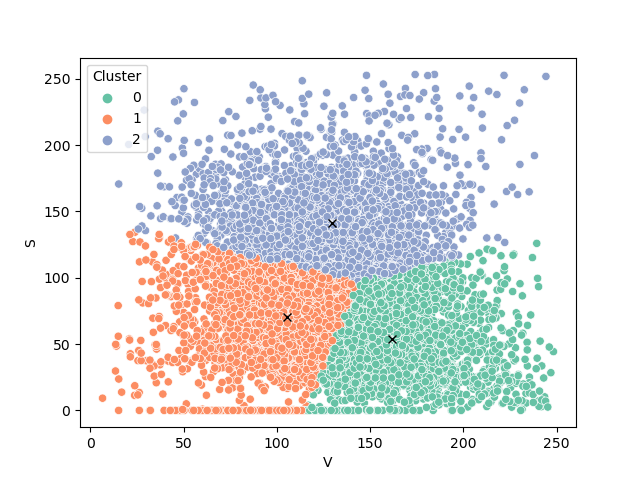
\includegraphics[width=1.0\textwidth]{cluster8.png}
	\label{Fig.42}
	\end{figure}

	\begin{figure}[htbp]
	\centering
	\caption{3类别数聚类,迭代次数为9时}
	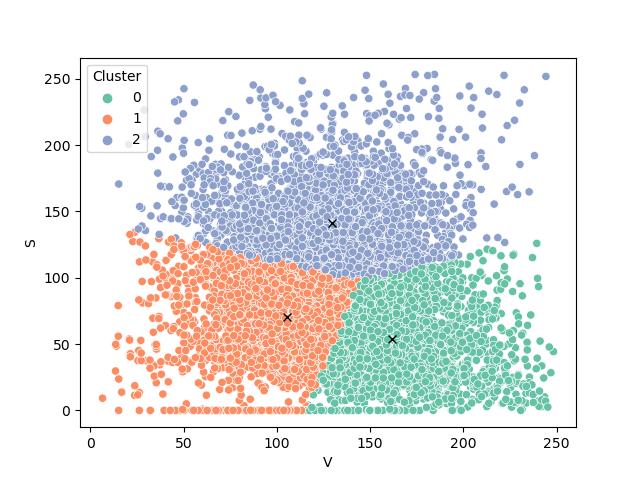
\includegraphics[width=1.0\textwidth]{cluster9.png}
	\label{Fig.43}
	\end{figure}

	\begin{figure}[htbp]
	\centering
	\caption{3类别数聚类,迭代次数为10时,聚类完成}
	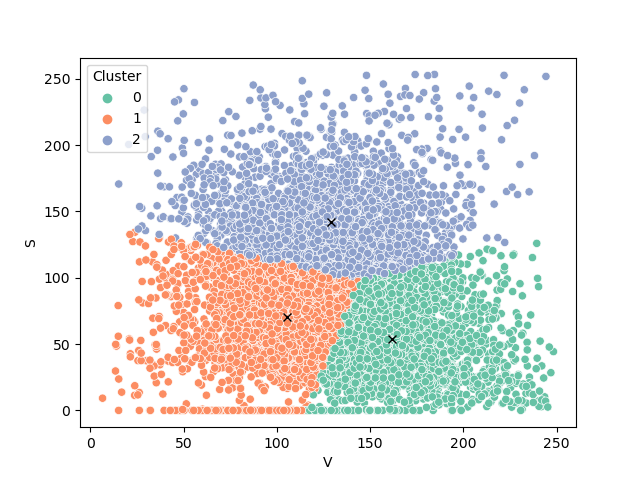
\includegraphics[width=1.0\textwidth]{cluster_final.png}
	\label{Fig.44}
	\end{figure}
	
	此外,我们也做出了聚类类别数为2和4时的聚类结果,分别如\hyperref[Fig.45]{图45}和\hyperref[Fig.46]{图46}所示。
	
	\begin{figure}[htbp]
		\centering
		\caption{2类别数聚类,迭代次数为7时,聚类完成}
		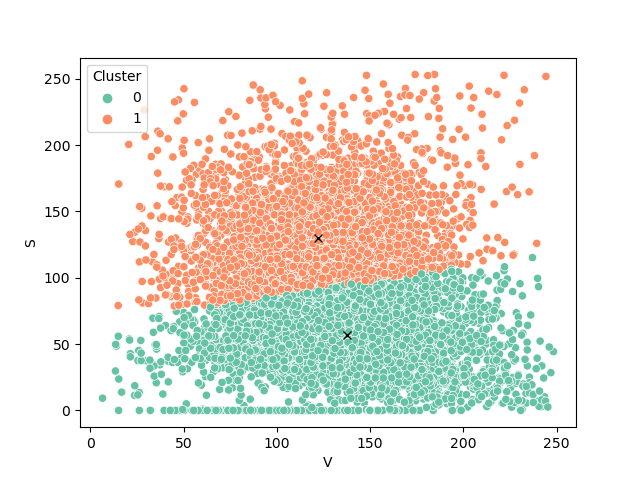
\includegraphics[width=1.0\textwidth]{cluster_final2.png}
		\label{Fig.45}
	\end{figure}

	\begin{figure}[htbp]
	\centering
	\caption{4类别数聚类,迭代次数为17时,聚类完成}
	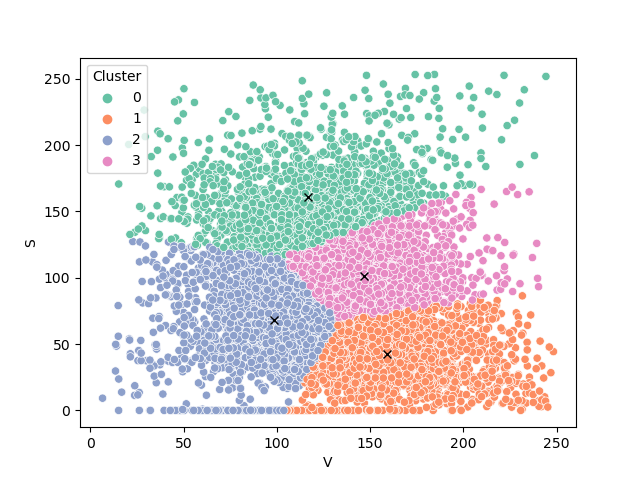
\includegraphics[width=1.0\textwidth]{cluster_final4.png}
	\label{Fig.46}
	\end{figure}

	\subsubsection{聚类结果分析}
	
	\begin{itemize}
		\item 当聚类类别数为2时,数据几乎被分成了上下两个部分,也即按照特征$S$的值是否大于75分成了2个簇。
		\item 当聚类类别数为3时,数据分成了上,左下和右下三个部分,也即先按照特征$S$是否大于125分成2类。是的部分单独为1个簇,不是的部分再按照特征$V$是否大于125分成两个簇。
		\item 当聚类类别数为4时,数据分成了上,左下,中右和右下四个部分。可以粗略地看作是在聚类类别为3的基础上,对于右下的簇再按照特征$S$是否大于60分成两个新的簇。
	\end{itemize} 
	
	
	\newpage \section{参考文献} 
	
	
	\begin{enumerate}
		\item Deng, J., Dong, W., Socher, R., Li, L. J., Li, K., \& Fei-Fei, L. (2009, June). Imagenet: A large-scale hierarchical image database. In 2009 IEEE conference on computer vision and pattern recognition (pp. 248-255). Ieee. \label{ref1}
		\item He, K., Zhang, X., Ren, S., \& Sun, J. (2016). Deep residual learning for image recognition. In Proceedings of the IEEE conference on computer vision and pattern recognition (pp. 770-778). \label{ref2}
	\end{enumerate}

	
\end{document}